% \documentclass[11pt, oneside]{article}      % use "amsart" instead of "article" for AMSLaTeX format


% \documentclass[submission,copyright,creativecommons]{eptcs}
% \providecommand{\event}{QPL 2021}

% \documentclass[runningheads]{llncs}

\documentclass[submission,copyright,creativecommons]{eptcs}
\providecommand{\event}{QPL 2022}
% \documentclass[submission,copyright,creativecommons]{eptcs}
% \providecommand{\event}{QPL 2021}

% \documentclass[runningheads]{llncs}

% \usepackage{geometry}                       % See geometry.pdf to learn the layout options. There are lots.
% \geometry{letterpaper}                          % ... or a4paper or a5paper or ... 
%\geometry{landscape}                       % Activate for rotated page geometry
%\usepackage[parfill]{parskip}          	% Activate to begin paragraphs with an empty line rather than an indent
\usepackage{graphicx}
\usepackage{amsmath,amsthm,amssymb}
\usepackage{mathtools}
\usepackage{xcolor}
\usepackage[font=small,labelfont=bf,skip=0pt,justification=justified]{caption}
\usepackage{stackengine}
% \usepackage{natbib}
\usepackage{stmaryrd}
\usepackage[most]{tcolorbox}
\usepackage{tikzit}
\input{zx.tikzdefs}
\input{zx.tikzstyles}

\usepackage{hyperref} % must be last package used

% \bibliographystyle{abbrvnat}
% \setcitestyle{square, authoryear}
% \setlength{\parindent}{0in}
% \setcitestyle{square}
\theoremstyle{definition}
\newtheorem{theorem}{Theorem}[section]
\newtheorem{corollary}[theorem]{Corollary}
\newtheorem{lemma}[theorem]{Lemma}
\newtheorem*{lemma*}{Lemma}
\newtheorem*{proposition*}{Proposition}
\newtheorem{proposition}[theorem]{Proposition}
\newtheorem{conjecture}[theorem]{Conjecture}
\newtheorem{definition}[theorem]{Definition}
\newtheorem{example}[theorem]{Example}
\newtheorem{remark}[theorem]{Remark}
\newtheorem{warning}[theorem]{Warning}

\newcommand{\defeq}{\vcentcolon=}
\newcommand{\eqdef}{=\vcentcolon}
\newcommand{\xeq}[1]{\mathrel{\stackon[5pt]{$=$}{$\scriptstyle{#1}$}}}
\newcommand{\xeqq}[2]{\mathrel{\stackon[5pt]{$=$}{\stackon[5pt]{$\scriptstyle{#1}$}{$\scriptstyle{#2}$}}}}
\newcommand{\abs}[1]{\ensuremath{\lvert #1 \rvert}}

\newcommand{\qutritZphase}[2]{\,\tikz{\node[style=qutrit Z phase] (x) {$#1$ \nodepart{lower} $#2$};}\,}
\newcommand{\qutritXphase}[2]{\,\tikz{\node[style=qutrit X phase] (x) {$#1$ \nodepart{lower} $#2$};}\,}

\newcommand{\qutritZspider}[2]{\,\begin{tikzpicture}
	\begin{pgfonlayer}{nodelayer}
		\node [style=none] (1) at (0, 0.75) {...};
		\node [style=none] (5) at (-0.75, 1) {};
		\node [style=none] (7) at (0.75, 1) {};
		\node [style=none] (8) at (0, -0.75) {...};
		\node [style=none] (9) at (-0.75, -1) {};
		\node [style=qutrit Z phase] (10) at (0, 0) {$#1$ \nodepart{lower} $#2$};
		\node [style=none] (11) at (0.75, -1) {};
	\end{pgfonlayer}
	\begin{pgfonlayer}{edgelayer}
		\draw [bend left=15] (10) to (11.center);
		\draw [bend right=15] (10) to (9.center);
		\draw [bend right=15] (10) to (7.center);
		\draw [bend left=15] (10) to (5.center);
	\end{pgfonlayer}
\end{tikzpicture}}
\newcommand{\qutritState}[3]{\, \begin{tikzpicture}
	\begin{pgfonlayer}{nodelayer}
		\node [style=none] (1) at (0, 0.75) {};
		\node [style=qutrit #1 phase] (2) at (0, -0.5) {$#2$ \nodepart{lower} $#3$};
	\end{pgfonlayer}
	\begin{pgfonlayer}{edgelayer}
		\draw (1.center) to (2);
	\end{pgfonlayer}
\end{tikzpicture}}
\newcommand{\qutritZstate}[2]{\qutritState{Z}{#1}{#2}}
\newcommand{\qutritXstate}[2]{\qutritState{X}{#1}{#2}}

\newcommand{\qubitPhaseGate}[2]{\,\begin{tikzpicture}
	\begin{pgfonlayer}{nodelayer}
		\node [style=#1 phase dot] (0) at (0, 0) {$#2$};
		\node [style=none] (1) at (0, 1) {};
		\node [style=none] (2) at (0, -1) {};
	\end{pgfonlayer}
	\begin{pgfonlayer}{edgelayer}
		\draw (1.center) to (2.center);
	\end{pgfonlayer}
\end{tikzpicture}}
\newcommand{\qubitZphase}[1]{\qubitPhaseGate{Z}{#1}}
\newcommand{\qubitXphase}[1]{\qubitPhaseGate{X}{#1}}

\newcommand{\someSpider}[1]{$\mathcal{#1}$-spider}
\newcommand{\someSpiders}[1]{\someSpider{#1}s}
\newcommand{\Mspider}[0]{\someSpider{M}}
\newcommand{\Nspider}[0]{\someSpider{N}}
\newcommand{\Pspider}[0]{\someSpider{P}}
\newcommand{\Mspiders}[0]{\someSpiders{M}}
\newcommand{\Nspiders}[0]{\someSpiders{N}}
\newcommand{\Pspiders}[0]{\someSpiders{P}}

\newcommand{\smallcolvec}[1]{\ensuremath{\begin{psmallmatrix}#1\end{psmallmatrix}}}

\newcommand{\qutritRuleFusion}{\hyperlink{qutrit_rule_fusion}{\mathbf{(f)}}}
\newcommand{\qutritRuleId}{\hyperlink{qutrit_rule_id}{\mathbf{(id)}}}
\newcommand{\qutritRuleTwist}{\hyperlink{qutrit_rule_twisted_cup}{\mathbf{(t)}}}
\newcommand{\qutritRuleZeroCopy}{\hyperlink{qutrit_rule_0_copy}{\mathbf{(cp_0)}}}
\newcommand{\qutritRuleBialgebra}{\hyperlink{qutrit_rule_bialgebra}{\mathbf{(b)}}}
\newcommand{\qutritRuleMCopy}{\hyperlink{qutrit_rule_m_copy}{\mathbf{(cp_{\mathcal{M}})}}}
\newcommand{\qutritRuleCommute}{\hyperlink{qutrit_rule_commute}{\mathbf{(cm)}}}
\newcommand{\qutritRuleHadamard}{\hyperlink{qutrit_rule_hadamard}{\mathbf{(H)}}}
\newcommand{\qutritRuleEuler}{\hyperlink{qutrit_rule_euler}{\mathbf{(E)}}}
\newcommand{\qutritRuleColourChange}{\hyperlink{qutrit_rule_colour_change}{\mathbf{(cc)}}}
\newcommand{\qutritRuleSnake}{\hyperlink{qutrit_rule_snake}{\mathbf{(s)}}}

\newcommand{\qubitRuleFusion}{\hyperlink{qubit_rule_fusion}{\mathbf{(f)}}}
\newcommand{\qubitRuleId}{\hyperlink{qubit_rule_id}{\mathbf{(id)}}}
\newcommand{\qubitRuleCopy}{\hyperlink{qubit_rule_copy}{\mathbf{(c)}}}
\newcommand{\qubitRulePi}{\hyperlink{qubit_rule_pi}{(\bf{\pi})}}
\newcommand{\qubitRuleBialgebra}{\hyperlink{qubit_rule_bialgebra}{\mathbf{(b)}}}
\newcommand{\qubitRuleHadamard}{\hyperlink{qubit_rule_hadamard}{\mathbf{(H)}}}
\newcommand{\qubitRuleColourChange}{\hyperlink{qubit_rule_colour_change}{\mathbf{(cc)}}}
\newcommand{\qubitRuleEuler}{\hyperlink{qubit_rule_euler}{\mathbf{(E)}}}
\newcommand{\eliminatePSpidersStatement}{
	Given any graph-like ZX-diagram containing an interior \Pspider\ $x$ with phase \qutritZphase{p}{p} for $p \in \{1,2\}$, suppose we perform a $p$-local complementation at $x$. Then the new ZX-diagram is related to the old one by the following equality:
	\begin{equation}
		\tikzfig{eliminate/P_spiders/bang/general/1} \quad = \quad \tikzfig{eliminate/P_spiders/bang/general/9}
	\end{equation}
}


\newcommand{\eliminateNSpidersStatement}{
	Given any graph-like ZX-diagram containing an interior \Nspider\ $x$ with phase \qutritZphase{0}{n} or \qutritZphase{n}{0} for $n \in \{1,2\}$, suppose we perform a $(-n)$-local complementation at $x$. Then, treating the two cases separately, the new ZX-diagrams are related to the old ones by the equalities:
	\begin{equation}
		\scalebox{0.8}{\tikzfig{eliminate/N_spiders/0_n/bang/general/1}} = 
		\scalebox{0.8}{\tikzfig{eliminate/N_spiders/0_n/bang/general/9}} ~~, \qquad
	% \end{equation*}
	% \begin{equation*}
		\scalebox{0.8}{\tikzfig{eliminate/N_spiders/n_0/bang/1}} =
		\scalebox{0.8}{\tikzfig{eliminate/N_spiders/n_0/bang/9}}
	\end{equation}
}


\newcommand{\eliminateMSpidersStatement}{
	Given any graph-like ZX-diagram containing two interior \Mspiders\ $i$ and $j$ connected by edge $ij$ of weight $w_{i,j} \eqdef w \in \{1,2\}$, suppose we perform a proper $\pm w$-pivot along $ij$ (both choices give the same result). For $w=1$, the new ZX-diagram is related to the old one by the following equality:
	\begin{equation}
		\begin{split}
			& \hspace{60pt} \scalebox{0.9}{\tikzfig{eliminate/M_spiders/bang/w_1/LHS}} \\[15pt]
		 	= &\quad \scalebox{0.9}{\tikzfig{eliminate/M_spiders/bang/w_1/RHS}}
		 \end{split}
	\end{equation}
	The case $w=2$ differs only as follows: in the first diagram (the left hand side of the equation), the edge $ij$ is purple (by definition), while in the lower diagram (the right hand side of the equation), a $\pm 2 = \mp 1$ will replace all occurences of $\pm 1$, and the roles of purple and blue will be swapped throughout.
}

\newcommand{\HEdgesAreModThreeStatement}{
	The following equations hold in the qutrit ZX-calculus:
	\begin{equation}
		\tikzfig{hadamard_lemmas/3_h_edges_vanish/blue} \ = \ 
		\tikzfig{hadamard_lemmas/3_h_edges_vanish/disconnected} \ = \ 
		\tikzfig{hadamard_lemmas/3_h_edges_vanish/purple} \ ,
		\hspace{25pt}
		\tikzfig{hadamard_lemmas/2_h_edges_flip/2_blue} \ = \ 
		\tikzfig{hadamard_lemmas/2_h_edges_flip/1_purple} \ ,
		\hspace{25pt}
		\tikzfig{hadamard_lemmas/2_h_edges_flip/2_purple} \ = \  
		\tikzfig{hadamard_lemmas/2_h_edges_flip/1_blue}
	\end{equation}
}

\newcommand{\qutritPivotEqualityStatement}{
	Given $a \in \mathbb{Z}_3$ and a graph state $(G, W)$ containing connected nodes $i$ and $j$, define $N_{=}(i, j) \defeq \left\{x \in N(i) \cap N(j) \mid w_{x,i} = w_{x,j} \right\}$ and $N_{\neq}(i, j) \defeq \left\{x \in N(i) \cap N(j) \mid w_{x,i} \neq w_{x,j} \right\}$. Then the following equation relates $G$ and its proper $a$-pivot along $ij$:
	\begin{equation}
		\tikzfig{graph_state/proper_local_pivot}
	\end{equation}
}

% \title{Classifying Complexity with the ZX-Calculus:\\
% Jones Polynomials and Potts Partition Functions}

\title{Simplification Strategies for the Qutrit ZX-Calculus}

\author{Alex Townsend-Teague $^{1, 3}$ and Konstantinos Meichanetzidis $^{1,2}$
	\institute{
		$^1$ Department of Computer Science, University of Oxford \\ 
		$^2$ Cambridge Quantum Computing Ltd. \\
		$^3$ Dahlem Center for Complex Quantum Systems, Freie Universit\"{a}t Berlin, 14195 Berlin, Germany}
	}
\def\titlerunning{Simplification Strategies for the Qutrit ZX-Calculus}
\def\authorrunning{Alex Townsend-Teague and Konstantinos Meichanetzidis}

% \def\titlerunning{Simplification strategies for the qutrit ZX-calculus}
% \def\authorrunning{A. Townsend-Teague and K. Meichanetzidis}

% \authorrunning{A. Townsend-Teague and K. Meichanetzidis}

\begin{document}
\maketitle
\begin{abstract}
	The ZX-calculus is a graphical language for suitably represented tensor networks, called ZX-diagrams.
	%, composed of primitive generators whose semantics are tensors over a (semi)ring.
	%By universality,
	%Any tensor network has a corresponding ZX-diagram.
	Calculations are done by transforming ZX-diagrams with rewrite rules.
	%, which preserve semantics, and two ZX-diagrams representing the same tensor can be transformed into each other \emph{only} by a sequence of rewrites.
	The ZX-calculus has found applications in reasoning about quantum circuits, condensed matter systems, quantum algorithms, quantum error correcting codes, and counting problems.
	A key notion is the stabiliser fragment of the ZX-calculus, a subfamily of ZX-diagrams for which rewriting can be done efficiently in terms of derived simplifying rewrites.
	% In quantum computation with qubits or of Boolean counting problems, one employs the qubit ZX-calculus.
	%	However, higher-dimensional cases are of interest as well.
	Recently, higher dimensional qudits have become more prominent in quantum computing.
	% , and there are counting problem families whose complexity depends on the dimension.
	The main contribution of this work is the derivation of
	efficient rewrite strategies for the stabiliser fragment of the qutrit ZX-calculus.
	This constitutes a first non-trivial step towards simplification of qutrit quantum circuits. We then give further interesting applications; we reinterpret known complexity-theoretic results about evaluating the Jones polynomial, an important link invariant in knot theory, and counting graph colourings.
\end{abstract}

\section{Introduction}



The ZX-calculus originates in
quantum foundations \cite{Coecke2011,vandewetering2020zxcalculus}.
It is a graphical language that allows for reasoning about ZX-diagrams,
%which are composed of primitive generators \cite{vandewetering2020zxcalculus} called `spiders'.
%A ZX-diagram is
which are interpreted as tensor networks over
a (semi)ring \cite{wang2020completeness}.
The calculus
is defined by a set of rewrite rules
%involving spiders. Performing a rewrite amounts to a
that transforming the diagrams.
Note that the set of rewrite rules \emph{depends} on
the (semi)ring over which they are interpreted.
Importantly, ZX rewrites are sound and complete.
%for linear maps over the chosen (semi)ring.


In the context of quantum computing,
the Gottesman-Knill theorem states that stabilizer quantum
circuits can be
simulated \emph{efficiently} on classical computers \cite{Aaronson2004},
where by simulation here we mean the \emph{exact} computation of quantum probability amplitudes.
An alternative
%- and in fact more general -
proof of the Gottesman-Knill theorem for qubits has been obtained graphically in terms of the qubit ZX-calculus.
Stabilizer circuits can be expressed by the \emph{stabilizer}
fragment of the ZX-calculus,
and stabilizer ZX-diagrams can be rewritten efficiently
in terms of derived rewrite strategies \cite{graph_theoretic_simplification}.
Moreover, these simplifying rewrites can be viewed as theorems
that are useful for simplifying or simulating universal quantum circuits, not just stabilizer circuits.
The key rewrite rules that enable the efficient rewriting
of qubit stabilizer ZX-diagrams
are called \emph{local complementation} and \emph{pivot},
the latter being a composition of three of the former \cite{graph_theoretic_simplification}.
In this work, we recall the \emph{qutrit} version of local complementation \cite{harny_completeness} and derive the corresponding pivot rule.
We then derive simplification strategies
which allow for the \emph{efficient} rewriting of qutrit stabilizer ZX-diagrams,
the core result of this work.

Interestingly, though the motivation for studying ZX diagrams stems from quantum computation, they have broader applicability as they
can express arbitrary linear maps;
every quantum circuit is a ZX-diagram but not vice versa.
A plethora of hard problems in physics and computer science
regard interacting many-body multi-state systems - both classical and quantum -
and reduce to \emph{exactly} computing a single scalar.
These range from quantum amplitudes,
partition functions in classical statistical mechanics,
counting problems, probabilistic inference, and many more.
Problem instances can be encoded as closed
tensor networks over an appropriate (semi)ring.
The scalar can be evaluated by \emph{full tensor contraction},
which in general is \#P-hard \cite{Damm2002},
and finding the optimal contraction path for a general tensor network is NP-hard.


If a scalar of interest is expressed as a closed ZX-diagram,
one can rewrite the diagram by applying rewrite rules; one's goal is then to perform \emph{full diagram simplification} in order to compute the desired scalar.
Again, simplifying arbitrary closed ZX-diagrams is \#P-hard and finding the optimal rewrite strategy is NP-hard.
Note that
given an arbitrary tensor network, one can attempt to invent rewrite rules by inspecting the contents of the tensors and performing linear-algebra operations \cite{gray2020hyperoptimized}.


ZX-diagrams have been leveraged to study the complexity of boolean satisfiability (SAT) and model counting (\#SAT) \cite{debeaudrap2020tensor}.
Model counting entails computing the number of satisfying assignments to a boolean formula,
% (given in conjunctive normal form)
and this number can be expressed as a closed diagram.
Specifically, one finds that in the case of XORSAT and \#XORSAT,
known to be tractable,
the corresponding ZX-diagrams representing the problems exactly correspond to qubit stabilizer diagrams.
Going further, the ZH calculus \cite{backens2018zh}, an equivalent language to ZX, can be imported to make graphically obvious
why 2SAT is in P but \#2SAT is \#P-complete, whereas 3SAT and \#3SAT are both hard.
The key realisation is that the decision problem is in fact a counting problem
but where the diagram is interpreted over the Boolean semiring.
Then the \emph{rewrite rules change accordingly} and quickly imply the above result by allowing efficient simplification strategies.

%Such observations make apparent the unifying power of diagrammatic reasoning for studying the complexity of problem families.  
% of universal interest,
% where the degrees of freedom are two-dimensional.
In the spirit of \cite{debeaudrap2020tensor}, we treat the ZX-calculus as a library of rewrite rules, from which we import the appropriate tools for the job depending on the occasion.
Here we present two case studies: evaluating the Jones polynomial at lattice roots of unity, and graph colouring.
Both of these problem families reduce to evaluating
closed tensor networks and show a transition in complexity
at a particular dimension, below which the tensor network corresponds to a stabilizer ZX-diagram.
We underline that throughout this work, all rewrites are valid
\emph{up to a scalar}
since we are only concerned about making statements about complexity.
Keeping track of multiplicative scalar factors that arise under diagram rewriting can be done efficiently.
%We are thus justified in omitting them for the purposes of this work.We also emphasise that the qutrit `elimination' rewrite rules we derive in Section \ref{sec:qutrits}\ have independent ramifications for circuit optimisation, though these are not explored here.

\section{Simplifying Qubit ZX-Diagrams}

In this section we briefly review the qubit ZX-calculus, recalling the definitions of graph-like diagrams and stabilizer diagrams.
Crucially, we also recall the simplifying rewrites that enable the efficient
simplification of stabilizer diagrams.

\subsection{The Qubit ZX-Calculus}

% Here we give a quick introduction to the qubit ZX-calculus.
The qubit ZX-calculus is a diagrammatic language for quantum processes generated by \emph{spiders}.
Spider legs, or \emph{wires}, represent vector spaces of dimension $d=2$.
Diagrams are read bottom-to-top; bottom open wires (not connected to anything) are \emph{input wires} and top ones are \emph{outputs}.
Diagrams with only outputs are called \emph{states} and those with only inputs are called \emph{effects}.
A \emph{closed} diagram is one with no input nor output wires
and it represents a scalar.

Spiders can be \emph{composed};
% output wires can be connected to input wires
% to form spider networks which are again valid ZX-diagrams.
placing diagrams side by side represents parallel composition ($\otimes$),
whose concrete interpretation is the tensor product.
Vertically stacking diagrams corresponds to sequential composition ($\circ$) and concretely it means matrix multiplication.
Specifically, it means tensor contraction of two spider tensors along the wires connecting them, i.e. the common tensor indices represented by these wires are summed over.
The concrete representation of these operations of course depends on the (semi)ring over which the spiders are interpreted as tensors.
For spiders $S$ and $S'$, we denote these as
\begin{equation}
\left\llbracket S \otimes S' \right\rrbracket = \left\llbracket S \right\rrbracket \otimes \left\llbracket S' \right\rrbracket ~~,\quad
	\left\llbracket S \circ S' \right\rrbracket = \left\llbracket S \right\rrbracket \cdot \left\llbracket S' \right\rrbracket 
\end{equation} 

%, so ZX-diagrams should be viewed as belonging to a formal language.

Spiders come in two species: green $Z$-spiders and red $X$-spiders, decorated by a \emph{phase} $\alpha\in[0,2\pi)$. When $\alpha=0$, we will omit it.
The \emph{standard representation} of the spider generators as tensors over $\mathbb{C}$ is:
\begin{equation}\label{eq:qubit_standard_interpretation}
	% \left\llbracket \ \tikzfig{qubit_spiders/Z_a_labelled} \ \right\rrbracket = 
	% \ket{0}^{\otimes m}\bra{0}^{\otimes n} + 
	% e^{i\alpha}\ket{1}^{\otimes m}\bra{1}^{\otimes n} ,
	% \quad
	% \left\llbracket \ \tikzfig{qubit_spiders/X_a_labelled} \ \right\rrbracket = 
	% \ket{+}^{\otimes m}\bra{+}^{\otimes n} + 
	% e^{i\alpha}\ket{-}^{\otimes m}\bra{-}^{\otimes n}
	\left\llbracket~ \scalebox{0.75}{\tikzfig{qubit_spiders/Z_a_labelled}} ~\right\rrbracket = 
	\ket{0}^{m}\bra{0}^{n} + 
	e^{i\alpha}\ket{1}^{m}\bra{1}^{n} ,
	~~
	\left\llbracket~ \scalebox{0.75}{\tikzfig{qubit_spiders/X_a_labelled}} ~\right\rrbracket = 
	\ket{+}^{m}\bra{+}^{n} + 
	e^{i\alpha}\ket{-}^{m}\bra{-}^{n}
\end{equation}
where $\{\ket{0}$, $\ket{1}\}$ is the \emph{$Z$-basis} and
$\ket{\pm}=\ket{0}\pm\ket{1}$ the \emph{$X$-basis} in $\mathbb{C}^2$, in Dirac notation.
The Hadamard gate $H$, whose function is to switch between the $Z$ and $X$ bases, is denoted as a yellow box.
Often we will instead draw a dashed blue line to represent a \emph{Hadamard edge}:
\begin{equation}
	\tikzfig{qubit_hadamard/yellow_box} \quad = \quad
	\tikzfig{qubit_hadamard/dashed} \quad = \quad
	\tikzfig{qubit_hadamard/decomposed} ~~~,
	\qquad 
	\left\llbracket ~~~ \tikzfig{qubit_hadamard/yellow_box} ~~~ \right\rrbracket \simeq 
	\ket{0}\bra{0}+\ket{0}\bra{1}+\ket{1}\bra{0}-\ket{1}\bra{1}
\end{equation}

The ZX-calculus is universal for multilinear maps;
any tensor over a (semi)ring has a corresponding ZX-diagram \cite{wang2020completeness}
.
The rewrite rules of the ZX-calculus (see Fig.\ref{fig:qubit_ZX_rules} in Appendix \ref{app:zx_calculus}) allow manipulation of the diagrams by \emph{local tensor-rewrites}. Importantly, up to a scalar, the rewrites are sound; they \emph{preserve the semantics}, i.e. the concrete tensor representation over $\mathbb{C}$.
The ZX-calculus is also \emph{complete} in the sense that any true equation between tensors can be proven \emph{only} in terms of rewrites;
the diagram on the left hand side of the equation can be transformed to that on the right hand side by applying rewrite rules.
This gives ZX the status of a `calculus'. 
What is important about qubit ZX-diagrams
is that \emph{only topology matters};
the concrete tensor semantics of the diagram are invariant under
deformations of the network as long as the inter-spider connectivity is respected.


\subsection{Stabilizer Qubit ZX Diagrams}

The \emph{stabilizer fragment} of the calculus consists of all diagrams in which all phases are $\alpha=\frac{\pi n}{2}$, $n\in\mathbb{Z}$.
%We note that both diagrams above fall into this stabilizer fragment. 
In (Theorem 5.4, \cite{graph_theoretic_simplification}) the authors give an efficient algorithm for simplifying any qubit ZX-diagram to an equivalent diagram with fewer spiders.
The algorithm consists of consecutive applications of spider-eliminating rewrites.

First it is shown that every diagram is equivalent to a \emph{graph-like} diagram:
every spider is green,
every edge is a Hadamard edge,
there are no parallel edges or self-loops,
every input and output wire is connected to a spider
and every spider has at most one input or output wire.
The following derivable rules are key to this:
\begin{equation}\label{eq:maintain_graph_like}
	\tikzfig{hadamard_lemmas/2_h_edges_vanish/lhs} \ = \  
	\tikzfig{hadamard_lemmas/2_h_edges_vanish/rhs} \ ,
	\hspace{50pt}
	\tikzfig{self_loop/plain/lhs} \ = \  
	\tikzfig{self_loop/plain/rhs} \ ,
	\hspace{50pt}
	\tikzfig{self_loop/hadamard/lhs} \ = \  
	\tikzfig{self_loop/hadamard/rhs}
\end{equation}
Then the following two rewrite rules, derived via
\emph{local complementation} and \emph{pivoting},
can be used to eliminate spiders:
	\begin{equation}\label{eq:eliminate_clifford}
		\tikzfig{eliminate/clifford}
	\end{equation}
	\begin{equation}\label{eq:eliminate_pauli}
		\tikzfig{eliminate/pauli}
	\end{equation}
For more details,
see (Section 4, \cite{graph_theoretic_simplification}).
Eq.~\eqref{eq:eliminate_clifford} says that we can remove any spider with phase $\pm\frac{\pi}{2}$ at the cost of performing a local complementation at said spider.
Furthermore,
Eq.~\eqref{eq:eliminate_pauli} says we can remove any pair of spiders with phases in $\{0, \pi\}$ connected by a Hadamard edge at the cost of performing a pivot along said edge.
After each application of \eqref{eq:eliminate_clifford} or \eqref{eq:eliminate_pauli}, we can use \eqref{eq:maintain_graph_like} to remove any parallel Hadamard edges and ensure the diagram remains graph-like.

In particular, and importantly to this work,
this algorithm will \emph{efficiently} simplify any closed stabilizer diagram until it contains at most one spider, at which point the scalar it represents can be easily read off. 
% If it exists, this spider is green, legless and has phase in $\{0, \pi\}$.
%We briefly outline the process here, referring the reader to \cite{graph_theoretic_simplification} for a full discussion.
% The point relevant to this work is that spiders can be \emph{eliminated efficiently}, i.e. with a polynomial number of rewrites in the initial number of spiders. 
By `efficiently' we mean via a sequence of spider elimination rewrites whose cost is polynomial in the initial number of spiders. Note each such rewrite updates only a polynomial number of edges in the diagram, which prevents an overwhelming memory cost of the simplification procedure.
\section{Simplifying Qutrit ZX-Diagrams}

We now turn to the qutrit ZX-calculus and examine the analogous story to that of the previous subsection
but now for the case where the dimension of the vector space carried by the wires is $d=3$.


\subsection{The Qutrit ZX-Calculus}


As in the qubit case, the qutrit ZX calculus concerns spiders connected by wires, but there are key differences, some subtler than others.
Again, spiders come in two species, Z (green) and X (red),
with the three-dimensional \emph{Z-basis} denoted as $\{\ket{0},\ket{1},\ket{2}\}$ .
% To get a feel for the qutrit calculus, we outline these differences briefly here before giving a formal definition. First of all, the qubit $Z$-basis consisted of two vectors $\ket{0} = \smallcolvec{1\\0}$ and $\ket{1} = \smallcolvec{0\\1}$, whereas the qutrit $Z$-basis consists of three vectors:
% \begin{equation}
% 	\ket{0} = \smallcolvec{1\\0\\0}, \hspace{20pt}
% 	\ket{1} = \smallcolvec{0\\1\\0}, \hspace{20pt}
% 	\ket{2} = \smallcolvec{0\\0\\1}. 
% \end{equation}
Let $\omega = e^{i \frac{2\pi}{3}}$ denote the third root of unity
with $\bar\omega = \omega^2$ its complex conjugate.
The qutrit \emph{$X$-basis} consists of the three vectors: 
\begin{equation}
	\ket{+} = \frac{1}{\sqrt{3}} \left(\ket{0} + \ket{1} + \ket{2}\right)~,~~
	\ket{\omega} = \frac{1}{\sqrt{3}} \left(\ket{0} + \omega\ket{1} + \bar{\omega}\ket{2}\right)~,~~
	\ket{\bar{\omega}} = \frac{1}{\sqrt{3}} \left(\ket{0} + \bar{\omega}\ket{1} + \omega\ket{2}\right)
\end{equation}
In qutrit ZX,
spiders carry \emph{two} phases $\alpha$ and $\beta$,
and have the following \emph{standard representation} as linear maps:
\begingroup
	\allowdisplaybreaks
	\setlength{\jot}{10pt}
		\begin{align}
			&\left\llbracket \quad \tikzfig{qutrit_generators/spiders/Z_a_b_labelled} \quad \right\rrbracket = 
			\ket{0}^{\otimes m}\bra{0}^{\otimes n} + 
			e^{i\alpha}\ket{1}^{\otimes m}\bra{1}^{\otimes n} + 
			e^{i\beta}\ket{2}^{\otimes m}\bra{2}^{\otimes n} \\
			&\left\llbracket \quad \tikzfig{qutrit_generators/spiders/X_a_b_labelled} \quad \right\rrbracket = 
			\ket{+}^{\otimes m}\bra{+}^{\otimes n} + 
			e^{i\alpha}\ket{\omega}^{\otimes m}\bra{\omega}^{\otimes n} + 
			e^{i\beta}\ket{\bar{\omega}}^{\otimes m}\bra{\bar{\omega}}^{\otimes n}
			% &\left\llbracket \quad \tikzfig{qutrit_generators/spiders/Z_a_b_labelled} \quad \right\rrbracket = 
			% \ket{0}^{\otimes m}\bra{0}^{\otimes n} + 
			% e^{i\alpha}\ket{1}^{\otimes m}\bra{1}^{\otimes n} + 
			% e^{i\beta}\ket{2}^{\otimes m}\bra{2}^{\otimes n} \\
			% &\left\llbracket \quad \tikzfig{qutrit_generators/spiders/X_a_b_labelled} \quad \right\rrbracket = 
			% \ket{+}^{\otimes m}\bra{+}^{\otimes n} + 
			% e^{i\alpha}\ket{\omega}^{\otimes m}\bra{\omega}^{\otimes n} + 
			% e^{i\beta}\ket{\bar{\omega}}^{\otimes m}\bra{\bar{\omega}}^{\otimes n}
		\end{align}
\endgroup
When $\alpha = \beta = 0$ we will again omit the angles entirely, and just draw a small green or red dot. Throughout our work, whenever we use an integer $n$ as a spider decoration, this is a shorthand for $\frac{2\pi}{3}n$. Since spider phases hold mod $2\pi$, these integer decorations hold mod $3$. Unless otherwise stated, we will use Greek letters to denote general angles, and Roman letters for these integer shorthands.
% This shouldn't ever cause confusion.

Hadamard gates are no longer self-adjoint, so we change our notation: we let a yellow box decorated with a $1$ (mod $3$) denote a Hadamard gate, while decorating with a $2$ (mod $3$) denotes its adjoint. We will shortly explain this choice. We also use a dashed blue line for the \emph{Hadamard edge} (\emph{$H$-edge}) and a purple dashed line for its adjoint (\emph{$H^\dagger$-edge}):
\begin{equation}\label{eq:qutrit_dashed_lines}
		\tikzfig{hadamard_lemmas/parametrised/1} \ = \ 
		\tikzfig{hadamard_lemmas/dashed/blue} \ = \ 
		\tikzfig{qutrit_rules/hadamard/euler/decomposition} ~~ , 
		\hspace{50pt}
		\tikzfig{hadamard_lemmas/parametrised/2} \ = \ 
		\tikzfig{hadamard_lemmas/dashed/purple} \ = \ 
		\tikzfig{hadamard_lemmas/decompositions/h_dagger_zxz} ~~ ,
		\hspace{50pt}
		\tikzfig{hadamard_lemmas/parametrised/0} \ = \ 
		\tikzfig{hadamard_lemmas/parametrised/empty}
\end{equation}

The last equation above just says that a \emph{$0$-Hadamard edge} is in fact the empty diagram, and not an edge at all. 
A very important difference from the qubit case is that in qutrit ZX-calculus there is no \emph{plain} cap or cup:
%. That is, we have the following two results:
\begin{equation}
	\tikzfig{cups_caps/z_cup} \quad \neq \quad \tikzfig{cups_caps/x_cup} \quad , \hspace{50pt}
	\tikzfig{cups_caps/z_cap} \quad \neq \quad \tikzfig{cups_caps/x_cap}
\end{equation}
This has several consequences. Firstly, the maxim that \emph{`only topology matters' no longer applies}. That is, it is now important to make clear the distinction between a spider's inputs and outputs, unlike in the qubit case where we could freely interchange the two. Diagram components can still be isotoped around the plane but only so long as this input/output distinction is respected. This gives the qutrit calculus a slightly more rigid flavour than its qubit counterpart. 
That said, this rigidity is loosened in certain cases; in particular, this distinction is irrelevant for $H$- and $H^\dagger$-edges \cite{qutrit_euler}:
% That said, this rigidity is loosened by the following two observations.
% Firstly, this distinction is irrelevant for $H$- and $H^\dagger$-edges \cite{qutrit_euler}:
	\begin{equation}
		\tikzfig{hadamard_lemmas/io_irrelevant/h/lhs} \ = \ 
		\tikzfig{hadamard_lemmas/io_irrelevant/h/rhs} \ ,
		\hspace{50pt}
		\tikzfig{hadamard_lemmas/io_irrelevant/h_dagger/lhs} \ = \ 
		\tikzfig{hadamard_lemmas/io_irrelevant/h_dagger/rhs}
	\end{equation}
% Secondly, the `snake equations' hold for \emph{same-colour} cups and caps.
% Snakes with differently coloured cups and caps can still be yanked into a straight wire at the cost of adding two Hadamard boxes, shown below for $h \in \{1, 2\}$:
% \begin{equation}
% 		\tikzfig{qutrit_snake/same_bent} \quad = \quad \tikzfig{qutrit_snake/same_straight} \quad ,
% 		\hspace{50pt}
% 		\tikzfig{qutrit_snake/different_bent} \quad = \quad \tikzfig{qutrit_snake/different_straight}
% \end{equation}
% The above equations hold also if we flip the colours, green $\leftrightarrow$ red. 
The full set of rules governing the qutrit ZX calculus is shown in Figure \ref{fig:qutrit_ZX_rules} in Appendix \ref{app:zx_calculus}.


\subsection{Graph-Like Qutrit ZX Diagrams}

% \numbered{Definition}{A \emph{Hadamard edge} (or \emph{H-edge}) is a Hadamard map connecting two spiders. A \emph{Hadamard adjoint edge} (or \emph{$H^\dagger$-edge) }}


A \emph{graph-like qutrit ZX diagram} is one where
every spider is green,
spiders are only connected by blue Hadamard edges (\emph{$H$-edges})
or their purple adjoints (\emph{$H^\dagger$-edges}),
every pair of spiders is connected by at most one $H$-edge or $H^\dagger$-edge,
every input and output wire is connected to a spider,
and every spider is connected to at most one input or output wire.
A graph-like qutrit ZX diagram is a \emph{graph state} when every spider has zero phase (top and bottom) and is connected to an output. 

% Thanks to Lemma \ref{lem:h_edges_input_output} we can ignore which of a spider's $H$- and $H^\dagger$-legs are inputs and outputs. For our specific needs, the last two items above will not be relevant, since ZX-diagrams arising from knots will be closed, but we include them to keep the definition consistent with the qubit case.

Note the difference compared to the qubit case: we need not worry about self-loops beacuse the qutrit ZX calculus doesn't define a `plain' cap or cup. But this comes at a cost: spiders in the qutrit case fuse more fussily. Specifically, when two spiders of the same colour are connected by at least one plain edge and at least one $H$- or $H^\dagger$-edge, fusion is not possible. Instead, we can ensure we have a graph-like diagram by replacing the plain wire:
% The following equation, for $h \in \{1,2\}$, helps us get around this:
% The following equation, which also holds with the roles of blue and purple interchanged, helps us get around this:
\begin{equation}\label{eq:spiders_reluctant_to_fuse}
	\tikzfig{hadamard_lemmas/plain_wire/1} \quad \xeq{\qutritRuleHadamard} \quad
	\tikzfig{hadamard_lemmas/plain_wire/2} \quad \xeq{\qutritRuleId} \quad
	\tikzfig{hadamard_lemmas/plain_wire/3} \quad = \quad
	\tikzfig{hadamard_lemmas/plain_wire/4}
\end{equation}

Indeed, we can show that every qutrit ZX-diagram is equivalent to a graph-like one. The following equations, derived in Appendix \ref{lem:h_edges_are_mod_3_appendix}, are vital to this:
\begin{equation}\label{eq:h_edges_are_mod_3}
	\tikzfig{hadamard_lemmas/3_h_edges_vanish/blue} \ = \ 
	\tikzfig{hadamard_lemmas/3_h_edges_vanish/disconnected} \ = \ 
	\tikzfig{hadamard_lemmas/3_h_edges_vanish/purple} \ ,
	\hspace{50pt}
	\tikzfig{hadamard_lemmas/2_h_edges_flip/2_blue} \ = \ 
	\tikzfig{hadamard_lemmas/2_h_edges_flip/1_purple} \ ,
	\hspace{50pt}
	\tikzfig{hadamard_lemmas/2_h_edges_flip/2_purple} \ = \  
	\tikzfig{hadamard_lemmas/2_h_edges_flip/1_blue}
\end{equation}

This justifies our notation for Hadamard gates: we can think of Hadamard edges as $1$-weighted edges and their adjoints as $2$-weighted edges, then work modulo $3$, since every triple of parallel edges disappears. Where the previous equations relate single $H$- and $H^\dagger$-boxes across multiple edges, the next three relate multiple $H$- and $H^\dagger$- boxes on single edges. They hold for $h \in \{1, 2\}$, and are proved via simple applications of rules $\qutritRuleId$, $\qutritRuleHadamard$ and $\qutritRuleSnake$.
\begin{equation}\label{eq:h_boxes_are_mod_4}
	\tikzfig{hadamard_lemmas/boxes/4_vanish} \quad ,
	\hspace{50pt}
	\tikzfig{hadamard_lemmas/boxes/3_flip} \quad ,
	\hspace{50pt}
	\tikzfig{hadamard_lemmas/boxes/2_separate}
\end{equation}

\begin{proposition}\label{prop:every_diagram_is_graph_like_qutrit}
	Every qutrit ZX diagram is equivalent to one that is graph-like.
	\begin{proof}
		First use the colour change rule to turn all X-spiders into Z-spiders. Then use \eqref{eq:h_boxes_are_mod_4} to remove excess $H$- and $H^\dagger$-boxes, inserting a spider between any remaining consecutive pair of such boxes, so that all spiders are connected only by plain edges, $H$-edges or $H^\dagger$-edges. Fuse together as many as possible, and apply \eqref{eq:spiders_reluctant_to_fuse} where fusion is not possible, so that no plain edge connects two spiders. Apply \eqref{eq:h_edges_are_mod_3} to all connected pairs of spiders until at most one $H$- or $H^\dagger$-edge remains between them. Finally, to ensure every input and output is connected to a spider and every spider is connected to at most one input or output, we can use $\qutritRuleHadamard$ and $\qutritRuleId$ to add a few spiders, $H$- and $H^\dagger$-edges as needed: 
		\begin{equation}
			\tikzfig{is_graph_like/plain_input_output_wire_coloured} \quad ,
			\hspace{50pt}
			\tikzfig{is_graph_like/input_connected_to_hadamard} \quad ,
			\hspace{50pt}
			\tikzfig{is_graph_like/multiple_inputs_connected_to_one_spider_coloured}
		\end{equation}
	\end{proof}
\end{proposition}

A graph state is described fully by its underlying multigraph, or equivalently by an adjacency matrix, where edges take weights in $\mathbb{Z}_3$\ (Lemma 4.2, \cite{harny_completeness}). Nodes correspond to phaseless green spiders, edges of weight $1$ correspond to Hadamard edges, and edges of weight $2$ correspond to $H^\dagger$ edges. As in the qubit case, graph states admit a \emph{local complementation} operation\ (Definition 2.6, \cite{harny_completeness}), though the effect is now slightly more complicated. We'll give the intuition after the formal definition:

\begin{definition}\label{def:local_complementation_qutrit}
	Given $a \in \mathbb{Z}_3$ and a graph state $G$ with adjacency matrix $W = (w_{i,j})$, the \emph{$a$-local complentation} at node $x$ is the new graph state $G *_a x$, whose adjacency matrix $W' = (w'_{i,j})$ is given by $w'_{i,j} = w_{i,j} + aw_{i,x}w_{j,x}$.
	% \begin{equation}
	% 	w'_{i,j} = w_{i,j} + aw_{i,x}w_{j,x}
	% \end{equation}
\end{definition}

So only those edges between neighbours of node $x$ are affected. Specifically, for two nodes $i$ and $j$ both connected to $x$ by the \emph{same} colour edge, $a$-local complementation at $x$ \emph{increases} weight $w_{i,j}$ by $a$. If instead $i$ and $j$ are connected to $x$ by edges of \emph{different} colours, $a$-local complementation at $x$ \emph{decreases} $w_{i,j}$ by $a$. This is shown graphically below, and holds with the roles of blue and purple interchanged:
\begin{equation}
	\tikzfig{a_local_comp/same}
	\hspace{75pt}
	\tikzfig{a_local_comp/different}
\end{equation}

% As in the qubit case, local complementation gives an equality up to introducing some single qubit phase gates on the outputs (Theorem 4.4, Corollary 4.5, \cite{harny_completeness}). 

\begin{theorem}\label{thm:local_comp_equality} (Theorem 4.4, Corollary 4.5, \cite{harny_completeness})~
	Given $a \in \mathbb{Z}_3$ and a graph state $(G, W)$ containing a node $x$, let $N(x)$ denote the neighbours of $x$; that is, nodes $i$ with weight $w_{i,x} \in \{1, 2\}$. Then the following equality holds:
	\ctikzfig{graph_state/local_comp}
\end{theorem}

% Composing local complementations gives a \emph{pivot} operation.

\begin{definition}\label{def:local_pivot_qutrit}
	Given $a,b,c \in \mathbb{Z}_3$ and a graph state $G$ containing nodes $i$ and $j$, the \emph{$(a,b,c)$-pivot} along $ij$ is the new graph state $G \wedge_{(a,b,c)} ij \defeq ((G *_a i) *_b j) *_c i$. 
\end{definition}

This pivot operation again leads to an equality, up to introducing some extra gates on outputs, whose proof is found in Appendix \ref{thm:local_pivot_equality_appendix}. Here we shall only consider an $(a,-a,a)$-pivot along an edge $ij$ of non-zero weight, for $a \in \{1, 2\}$. We will call this a \emph{proper $a$-pivot} along $ij$, and denote it $G \wedge_a ij$.

\begin{theorem}\label{thm:local_pivot_equality}
	Given $a \in \mathbb{Z}_3$ and a graph state $(G, W)$ containing connected nodes $i$ and $j$, define $N_{=}(i, j) \defeq \left\{x \in N(i) \cap N(j) \mid w_{x,i} = w_{x,j} \right\}$ and $N_{\neq}(i, j) \defeq \left\{x \in N(i) \cap N(j) \mid w_{x,i} \neq w_{x,j} \right\}$. Then the following equation relates $G$ and its proper $a$-pivot along $ij$:
	% Given $a \in \mathbb{Z}_3$ and a graph state $(G, W)$ containing connected nodes $i$ and $j$, define the following:
	% \begin{itemize}
	% 	\item $N_{=}(i, j) \defeq \left\{x \in N(i) \cap N(j) \mid w_{x,i} = w_{x,j} \right\}$
	% 	\item $N_{\neq}(i, j) \defeq \left\{x \in N(i) \cap N(j) \mid w_{x,i} \neq w_{x,j} \right\}$
	% \end{itemize} 
	% Then the following equation relates $G$ and its proper $a$-pivot along $ij$:
	\ctikzfig{graph_state/proper_local_pivot}

	% \begin{proof}
	% 	See Appendix \ref{thm:local_pivot_equality_appendix}.
	% \end{proof}
\end{theorem}

\subsection{Qutrit Elimination Theorems}

We classify spiders into three families exactly as in (Theorem 3.1, \cite{harny_completeness}):
\begin{equation}
	\mathcal{M} = \left\{\qutritZspider{0}{0}, \qutritZspider{1}{2}, \qutritZspider{2}{1}\right\},
	\hspace{10pt}
	\mathcal{N} = \left\{\qutritZspider{0}{1}, \qutritZspider{1}{0}, \qutritZspider{0}{2}, \qutritZspider{2}{0}\right\},
	\hspace{10pt}
	\mathcal{P} = \left\{\qutritZspider{1}{1}, \qutritZspider{2}{2}\right\}.
\end{equation}
We call a spider in a graph-like ZX-diagram \emph{interior} if it isn't connected to an input or output. Given any graph-like ZX-diagram, we will show that we can eliminate standalone interior $\mathcal{P}$- and \Nspiders\ by local complementation, and pairs of connected interior \Mspiders\ by pivoting. 

First, we define (a very small extension of) the \emph{!-box} notation (pronounced \emph{`bang-box'}), as introduced in \cite{dixon2009graphical} for general string diagrams. A !-box in a ZX-diagram allows its contents to `unfold' out arbitrarily; that is, the contents of the !-box, along with any wires into or out of the box, can be copied $n$ times for any non-negative integer $n$, and placed side-by-side. Following the style of \cite{backens2018zh}, we also allow a parameter over which a !-box unfolds. We extend this notation as follows: in the corner of the !-box we allow a small further diagram, which denotes that the unfolded diagrams should all be pairwise connected by the diagram in the corner of the box. The simplest choice of this `corner diagram' is just the plain wire. In qutrit ZX-diagrams this notation will only be well-defined in certain scenarios: in particular, it is well-defined when the corner diagram is a $H$- or $H^{\dagger}$-edge (since then the distinction between a spider's input and output wires disappears) and the main contents of the !-box is equivalent to a single spider (since then there is no ambiguity about which spiders are connected by the corner diagram). For example, letting $[K] = \{1, ..., K\}$, we have: 
\begin{equation*}
	\left\{ \tikzfig{bang/connected/K} ~ : ~ K \in \{0, 1, 2, 3, ...\} \right\} = \ 
	% \left( \ 
	% 	\tikzfig{bang/connected/bang_0} \ , \
	% 	\tikzfig{bang/connected/bang_1} \ , \ 
	% 	\tikzfig{bang/connected/bang_2} \ , \ 
	% 	\tikzfig{bang/connected/bang_3} \
	% \right) \ = \ 
	\left\{ ~
		\tikzfig{bang/connected/0} \quad , \quad
		\tikzfig{bang/connected/1} \quad , \quad
		\tikzfig{bang/connected/2} \quad , \quad
		\tikzfig{bang/connected/3} \quad , \ ... 
	~ \right\}
\end{equation*}

\begin{theorem}\label{thm:eliminate_P_spiders}
	\eliminatePSpidersStatement
\end{theorem}

\begin{theorem}\label{thm:eliminate_N_spiders}
	\eliminateNSpidersStatement
\end{theorem}

\begin{theorem}\label{thm:eliminate_M_spiders}
	\eliminateMSpidersStatement
\end{theorem}

Proofs of these theorems are found in Appendix \ref{thm:eliminate_P_spiders_appendix}, \ref{thm:eliminate_N_spiders_appendix} and \ref{thm:eliminate_M_spiders_appendix} respectively. We can now combine them into an algorithm for efficiently simplifying a \emph{closed} graph-like ZX-diagram. First note that after applying any one of the three elimination theorems to such a diagram, and perhaps removing parallel $H$- or $H^\dagger$-edges via \eqref{eq:h_edges_are_mod_3}, we again have a graph-like diagram.

\begin{theorem}\label{thm:simplification_algorithm_works}
	Given any closed graph-like ZX-diagram, the following algorithm will always terminate after a finite number of steps, returning an equivalent graph-like ZX-diagram with no \Nspiders, \Pspiders, or adjacent pairs of \Mspiders. Repeat the steps below until no rule matches. After each step, apply \eqref{eq:h_edges_are_mod_3} as needed until the resulting diagram is graph-like:
	\begin{enumerate}
		\item Eliminate a \Pspider\ via Theorem~\ref{thm:eliminate_P_spiders}.
		\item Eliminate an \Nspider\ via Theorem~\ref{thm:eliminate_N_spiders}.
		\item Eliminate two adjacent \Mspiders\ via Theorem~\ref{thm:eliminate_M_spiders}.
	\end{enumerate}
	\begin{proof}
		At every step the total number of spiders decreases by at least one, so since we start with a finite diagram the algorithm terminates after a finite number of steps. By construction, when it does so we are left with an equivalent graph-like ZX-diagram with no \Nspiders, \Pspiders, or adjacent pairs of \Mspiders.
	\end{proof}
\end{theorem}

In particular, if we start with a stabilizer diagram, we can eliminate all but perhaps one spider, depending on whether the initial number of \Mspiders\ was odd or even. This is because no step introduces any non-stabilizer phases. The algorithm above could be extended to a \emph{non-closed} graph-like diagrams as in (Theorem 5.4, \cite{graph_theoretic_simplification}) - for example, as part of a qutrit circuit optimisation algorithm. However, since this paper focuses on using the ZX-calculus to simplify \emph{closed} tensor networks, we have not done so.
\section{Case studies}

In this section we present two problems which can naturally be cast in tensor network form.
These problem families are interesting in that they show a transition in complexity when the dimension $d$ carried by the wires of the network is greater than a specific value. The \emph{Jones polynomial} is a prominent \emph{link invariant} in knot theory; here we present the problem of evaluating it at the \emph{lattice roots of unity}.
Subsequently, we briefly look at graph colouring.

\subsection{Jones Polynomial at Lattice Roots of Unity}

% For $d=2,3,4$ it's easy.
% For $d\geq 5$ it's hard.
% Mention Potts and also anyon stuff but the important thing is the tensornet.

A \emph{knot} $K$ is a circle embedded in $\mathbb{R}^3$.
A set of knots tangled together make a \emph{link} $L$.
A link $L$ can be represented by a \emph{link diagram}
by projecting it on to the plane
but retaining the information of \emph{over or under crossings}.
% For example, the trefoil knot linked with an unknot can be drawn as:
% \begin{equation}
% 
\includegraphics[scale=0.2]{figures/link.jpg}
% \label{eq:link}
% \end{equation}
We say that $L\simeq L'$ iff the diagram of link $L$ can be deformed to that of link $L'$ without cutting or gluing strands, or passing strands through each other.
% there is a sequence of Reidemeister moves from $L$ to $L'$, i.e. reversible local strand deformations that do not change the topology, for example by cutting or gluing strands (see Appendix).
The Jones polynomial $V_L(t)$
is a Laurent polynomial in a variable $t\in\mathbb{C}$
and is a \emph{link invariant}.
This means that
$V_L(t)\neq V_{L'}(t)\Rightarrow L\not\simeq L'$.

In general, computing $V_L(t)$
is exponentially costly in the number of crossings $c$,
something made explicit when one uses the Kauffman bracket method \cite{Kauffman2001}.
Exactly evaluating the Jones polynomial at points $t\in\mathbb{C}$ is \#P-hard,
\emph{except} at the \emph{lattice roots of unity} $\Lambda = \{ \pm 1, \pm i, \pm e^{i 2\pi/3}, \pm e^{i 4\pi/3} \}$,
where it can be evaluated at cost $O(poly(c))$ \cite{jaeger_vertigan_welsh_1990}.


In the context of quantum computation,
additively approximating the Jones polynomial at \emph{non-lattice roots of unity} is the paradigmatic BQP-complete complete problem \cite{Aharonov_2008,kuperberg2014hard}.
Topological quantum computation \cite{Freedman2002,pachos_2012} is the most natural model for such knot theoretic questions. In this model, quantum states are defined in the fusion space of \emph{non-abelian anyons}, emergent quasiparticles with nontrivial exchange statistics arising in two-dimensional exotic phases of matter.
Quantum computation is performed by creating anyons from the vacuum, then braiding them, and finally fusing them back to the vacuum, where braids play the role of unitary gates.
The world-lines of the anyons define a closed braid, i.e. a link.
Such a link encodes a quantum amplitude corresponding to its Jones polynomial evaluated at a root of unity depending on the anyon theory at hand \cite{Witten1989}. 
Specifically, in the case of $\text{SU}(2)_k$ anyons, the Jones polynomial is evaluated at $t(k) = e^{i 2\pi/(2+k)}$ \cite{Rowell_2018}.

Remarkably, the evaluation of the Jones polynomial at certain points can be expressed as an unphysical partition function $Z_{G_L}(d)$ of a $d$-state Potts model with suitable spin-spin interactions \cite{RevModPhys.64.1099}.
This Potts model is defined on a signed graph $G_L$, obtained as follows.
The link diagram is bicoloured checkerboard-style,
then every coloured area is mapped to a vertex and every crossing is mapped to a signed edge according
its orientation relative to the surrounding colours, as in \eqref{eq:link-tn} below.
The Jones polynomial is then equal to this partition function up to an efficiently computable scalar which depends on the link diagram.  
% $V_L(t(d)) \simeq Z_{G_L}(d)$.
The relation between the point $t(d)$ at which the Jones polynomial is evaluated and the dimension $d$ of the spins is $d = t + t^{-1} +2$,
which can be solved for $t(d)$ \cite{PhysRevE.100.033303}.

Note the correspondence between the dimension $d$ in the Potts approach and the level $k$ in the anyon-braiding approach to the Jones polynomial: $\{t(d) | ~ d \in\{1,2,3,4\} \} = \{ t(k) | ~ k\in\{1,2,4,\infty\} \} \subseteq \Lambda$.
This is consistent with the fact that braiding $\text{SU}(2)_2$ anyons (Ising) or $\text{SU}(2)_4$ anyons is not universal (unless the $\text{SU}(2)_4$ anyons are augmented by fusion and measurements \cite{Levaillant_2015}).
% A key observation is that if $d\in\{2,3,4\}$ then $t(d)\in\Lambda$ (the case $d=1$ is trivial \cite{jaeger_vertigan_welsh_1990}).

The partition function $Z_{G_L}(d\in\mathbb{N})$ can be expressed as a closed tensor network in terms of phaseless (green) $d$-dimensional $Z$-spiders connected via wires that go through \emph{$\pm$-boxes} \cite{PhysRevE.100.033303}:
\begin{equation}
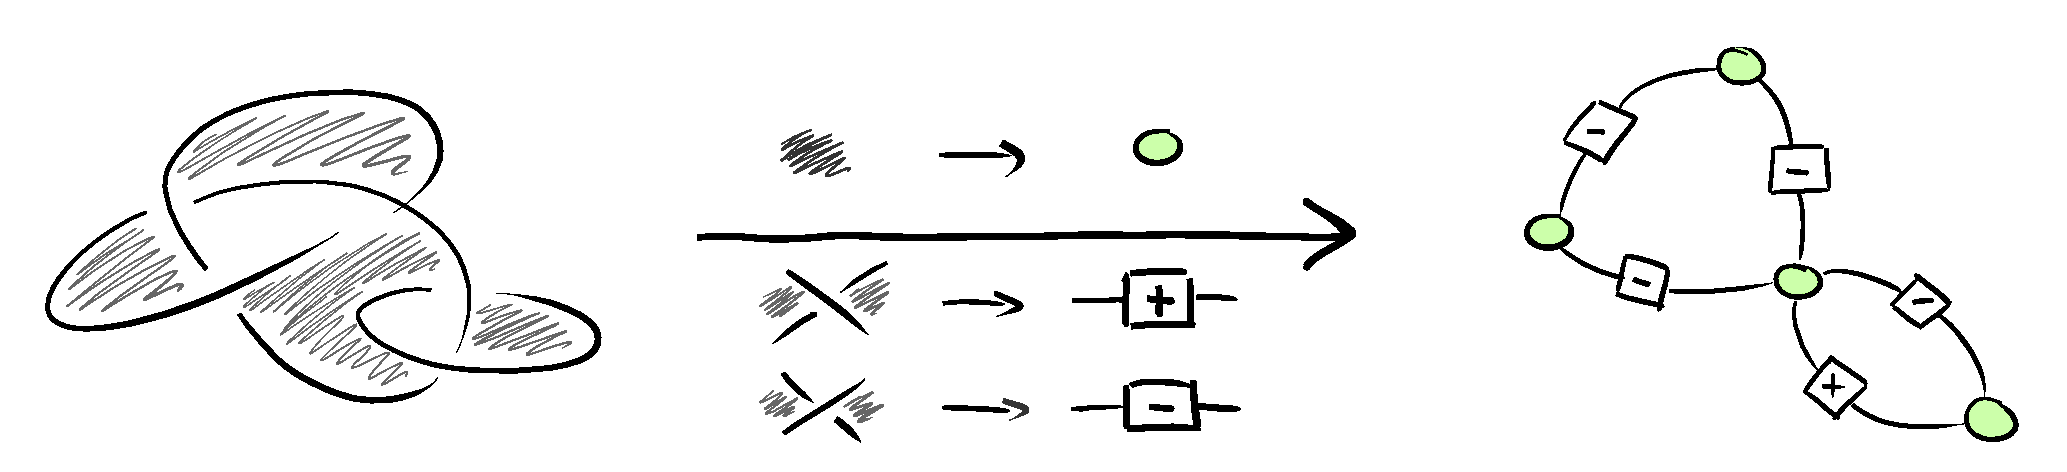
\includegraphics[scale=0.4, valign=c]{figures/link-tn.pdf}
\label{eq:link-tn}
\end{equation}
The $\pm$-boxes have the following concrete interpretation as matrices:
\begin{equation}\label{eq:pm_tensor}
	\left\llbracket \ \tikzfig{pm_maps/pm} \ \right\rrbracket ~~ = ~~  
	\sum_{i,j=0}^{d-1}(1 - (1+t(d)^{\mp 1}) \delta_{ij} ) \ket{i}\bra{j} ~~ = ~~  
	\begin{pmatrix}
		-t(d)^{\mp 1} & 1 & \dots & 1 \\
		1 & -t(d)^{\mp 1} & \dots & 1 \\
		\vdots & \vdots & \ddots & \vdots\\
		1 & 1 & \dots & -t(d)^{\mp 1}
	\end{pmatrix}
\end{equation}
% \begin{remark}\label{rem:qubit_scalar_exactness} 
% 	A small technical remark is in order: the rule set given here is complete for qubit stabilizer quantum mechanics when equality is taken only up to a scalar factor. To achieve completeness under exact equality, a slighly modified rule set would be required, as in (for example) \cite{backens_scalar_exact}. But for our purposes this would be overkill; in order to show that the Jones polynomial of knots at lattice roots of unity is efficiently computable, it suffices to consider the `non-exact' rules - i.e. it suffices to show such a Jones polynomial is efficiently computable up to a scalar factor. But of course to actually compute such a Jones polynomial, we would need to keep track of scalars.
% \end{remark}
% [Move commented out stuff below to appendix proof?]
% DON"T DELETE!!!!!!!!!!!!!!!!!!!!!!!
 % This is because the standard interpretation of diagrams more complex than a single spider can be derived as follows. First a diagram is divided into horizontal strips, then these strips are themselves divided vertically, so that the diagram consists of spiders composed in parallel (side-by-side, written $\otimes$) and in sequence (on top of each other, with legs fused together, written $\circ$). Such a division always exists, though it may require a diagram deformation. For example:
% For spiders $S$ and $T$, we then have:
% \begin{equation}
% 	\left\llbracket S \otimes T \right\rrbracket = \left\llbracket S \right\rrbracket \otimes \left\llbracket T \right\rrbracket 
% \end{equation} 
% \begin{equation}	
% 	\left\llbracket S \circ T \right\rrbracket = \left\llbracket S \right\rrbracket \left\llbracket T \right\rrbracket 
% \end{equation} 
% where on the right hand side of the first equation the $\otimes$ symbol means the Kronecker product of two matrices. Thus a diagram with standard interpretation $T_{2\pm}$ will have one input and one output, while a diagram for $T_{4\pm}$ will have two inputs and two outputs.



We can now express the $\pm$-boxes in the ZX-calculus.
The $\pm$-matrices above for $d \in \{2, 4\}$
are equal up to a scalar to concrete interpretations of \emph{qubit stabilizer} ZX-diagrams, and the $\pm$-matrices for $d=3$ of \emph{qutrit stabilizer} ZX-diagrams (see Appendix \ref{prop:pm_maps_zx_appendix}):
	\begin{equation}
		\left\llbracket \ \tikzfig{pm_maps/pm} \ \right\rrbracket_{d=2} \simeq 
		\left\llbracket \ \tikzfig{pm_maps/q2} \ \right\rrbracket ~, 
		\hspace{30pt}
		\left\llbracket \ \tikzfig{pm_maps/pm} \ \right\rrbracket_{d=3} \simeq
		\left\llbracket \ \tikzfig{pm_maps/q3} \ \right\rrbracket ~,
		\hspace{30pt}
		\left\llbracket \ \tikzfig{pm_maps/pm} \ \right\rrbracket_{d=4} \simeq 
		\left\llbracket \ \tikzfig{pm_maps/q4} \ \right\rrbracket
	\end{equation}
Since these generators decompose as stabilizer diagrams,
$Z_{G_L}(d\in\{2,3,4\})$ can be evaluated \emph{efficiently}
via stabilizer ZX-diagram simplification.
Thus, we recover the known result that evaluating the Jones polynomial at $t\in\Lambda$ is in P.
Computing $Z_{G_L}(d\geq 5)$ is \#P-hard.

%%%%%%%%%%%%%%%%%$ MAYBE SAVE DISCUSSIONS ABOUT WHAT THE SCALAR IS FOR WHEN WE DO THE SCALAR-EXACT VERSION %%%%%%%%%%%%%%%%%%
% Since any ZX-diagram derived from a knot in the manner described in Section \ref{sec:passage} will be closed, this algorithm suffices to prove that the calculation of the Jones polynomial of any knot at the lattice roots of unity $\pm 1$ and $\pm i$ is efficient. This is because reading off the scalar at the end is trivial; either we have the empty diagram, which has standard interpretation $1$, or a single legless $Z$-spider with phase $k\pi$:
% \begin{equation}
% 	\left\llbracket \ \tikzfig{scalars/Z_kpi_1} \ \right\rrbracket = 
% 	\left\llbracket \ \tikzfig{scalars/Z_kpi_2} \ \right\rrbracket = 
% 	( \bra{0} + \bra{1} )( \ket{0} + e^{ik\pi}\ket{1} ) =
% 	1 + e^{ik\pi}
% \end{equation}
% {\bf Furthermore, keeping track of the scalar factors introduced with each application of Theorem \ref{thm:qubit_eliminate_spiders} or Lemma \ref{lem:2_h_edges_vanish} can be done efficiently. [ToDo: proof, if not explicitly doing all this in a scalar-exact fashion. Reference Backens]}

% Having defined the \emph{qutrit} ZX-calculus, we turn our attention back to our tensor network for the Jones polynomial of a knot (ToDo: ref). We are seeking a diagram in the qutrit ZX-calculus that equals (up to a scalar) the matrix $T_{\pm}^{(q)}$ from \eqref{eq:pm_tensor}.

% where we have used $t = \frac{1}{2}(3 - 2 + \sqrt{3(3-4)}) = e^{i\frac{\pi}{3}}$ as in (ToDo: ref). 

% \begin{proposition}\label{prop:pm_map_q3}
% 	Under the standard interpretation as a linear map, the following diagram gives (up to a scalar) the required matrix:
% 	\begin{equation}
% 		\left\llbracket \quad \tikzfig{pm_maps/q3} \quad \right\rrbracket  \simeq
% 		% 2\sqrt{3}e^{\mp i\frac{5\pi}{6}} \ 
% 		\left\llbracket \quad \tikzfig{pm_maps/pm} \quad \right\rrbracket_{q=3} = 
% 		\begin{pmatrix}
% 			e^{\mp i\frac{\pi}{3}} & 1 & 1 \\
% 			1 & e^{\mp i\frac{\pi}{3}} & 1 \\
% 			1 & 1 & e^{\mp i\frac{\pi}{3}} \\
% 		\end{pmatrix}
% 	\end{equation}

% 	\begin{proof}
% 		See Appendix \ref{prop:pm_maps_zx_appendix}.
% 	\end{proof}
% \end{proposition}

% Crucially, the ZX-diagram in Proposition \ref{prop:pm_map_q3} above is a \emph{stabilizer diagram} in the qutrit ZX-calculus - that is, all angles are integer multiples of $\frac{2\pi}{3}$. Therefore if we can find an algorithm analogous to Theorem 5.4 \cite{graph_theoretic_simplification} that efficiently reduces any stabilizer diagram to a trivial one, then we will have shown that the Jones polynomial of any knot at the lattice roots of unity $\pm e^{i\frac{\pi}{3}}$ is efficiently computable. [ToDo: justify the $\pm$]. In the next subsection, we will do exactly that.

% Again - just like in Remark~\ref{rem:qubit_scalar_exactness} - these rules are complete for qutrit stabilizer quantum mechanics when equality is considered only up to a scalar factor; we give the scalar-exact versions (detailed in \citep{qutrit_exact}) so that we can actually compute Jones polynomials later. 




\subsection{Graph Colouring}


Finally, let us briefly look at the \emph{graph colouring problem}. A \emph{$d$-colouring} of a graph $G$ is an assignment of colours $\{1, ..., d\}$ to the vertices of $G$ so that no neighbouring vertices have the same colour. Given a graph $G$ and an integer $d$, we wish to \emph{count} the number of such $d$-colourings. Again, this problem can be interpreted as the zero-temperature
partition function of an antiferromagnetic Potts model (there is an energy cost for adjacent spins to be in the same state).
Through the lens of our graphical exposition we see that counting problems and computing partition functions are essentially the same problem, since both can be straightforwardly encoded as closed tensor networks.

Given a graph $G$, the graph colouring problem can be encoded as a ZX-diagram as follows. Every vertex of the graph is mapped to a $d$-dimensional phaseless (green) $Z$-spider.
Every edge is mapped to a wire connecting the spiders
which goes through an $X$-box.
\begin{equation}\label{eq:G-tn}
	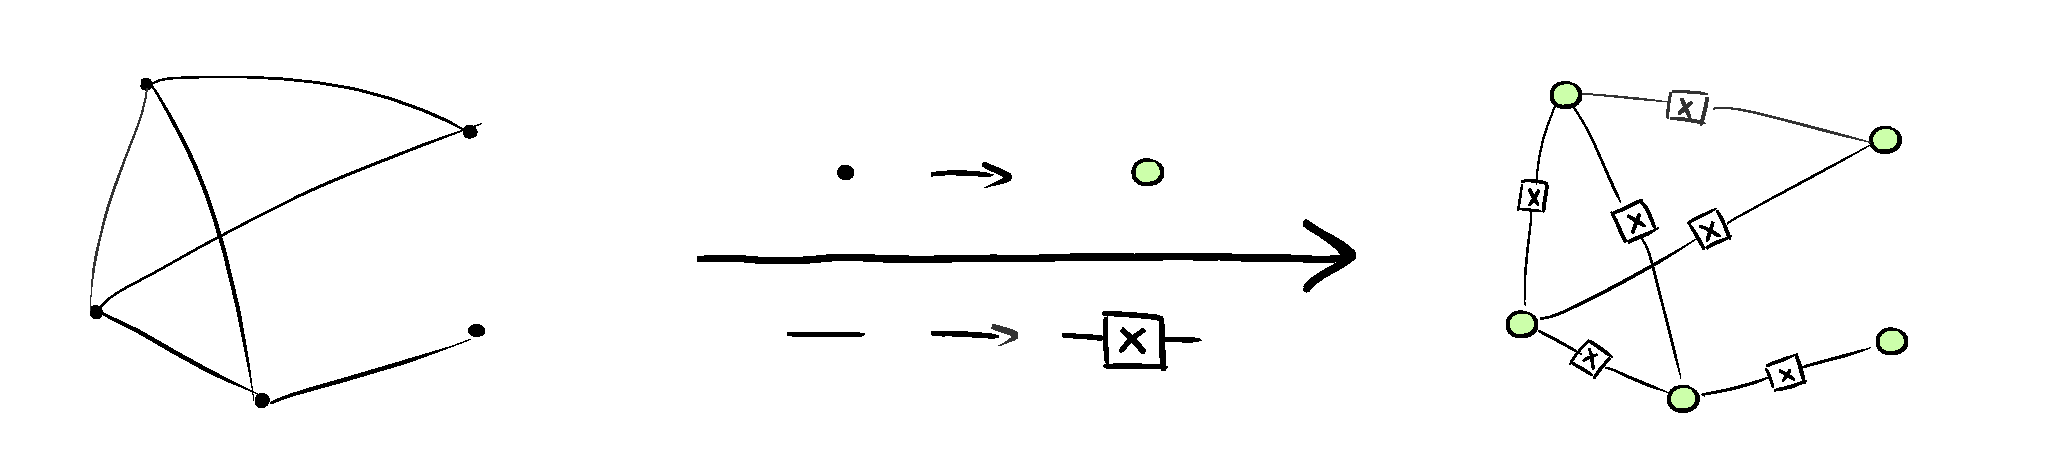
\includegraphics[scale=0.4, valign=c]{figures/G-tn.pdf}
\end{equation}
The $X$-boxes have the following concrete interpretation (as special case of the $\pm$-boxes, where $t=0$):
\begin{equation}\label{eq:X_tensor}
	\left\llbracket \ \tikzfig{pm_maps/x} \ \right\rrbracket ~~ = ~~  
	\sum_{i,j=0}^{d-1} (1 -  \delta_{ij} ) \ket{i}\bra{j} ~~ = ~~  
	\begin{pmatrix}
		0 & 1 & \dots & 1 \\
		1 & 0 & \dots & 1 \\
		\vdots & \vdots & \ddots & \vdots\\
		1 & 1 & \dots & 0
	\end{pmatrix}
\end{equation}

Counting k-colourings for $k\geq 3$ is a canonical \#P-complete problem,
while for $k=0,1,2$ the problem is in P \cite{jaeger_vertigan_welsh_1990}.
And indeed, for $d=2$ the $X$-matrix is just the Pauli X, and so the problem reduces to simplifying a stabilizer diagram,
which can be done efficiently.
	\begin{equation}\label{eq:XmatricesinZX}
		\left\llbracket \ \tikzfig{pm_maps/x} \ \right\rrbracket_{d=2} \simeq \left\llbracket \ \tikzfig{pm_maps/q2x} \ \right\rrbracket
	\end{equation}
However, for $d=3$ the $X$-matrix cannot be expressed as a stabilizer qutrit diagram; we prove this using our qutrit elimination theorems in Appendix \ref{prop:X_box_not_stab}. Thus it is not expected that there exists an efficient simplification strategy for the corresponding qutrit ZX-diagram. This is consistent with the fact that counting 3-colourings is \#P-complete.

\section{Outlook}

In this work, we have advocated for the use of the ZX-calculus
as a convenient graphical framework for treating a broad range of many-body problems on equal footing, and for diagnosing the complexity of interesting families of problems.
When the solution to a problem is encoded as a closed ZX-diagram,
this solution can be obtained via full diagram simplification by applying the rules of the calculus.
The problem can be solved \emph{efficiently} when the diagram encoding its answer is in the stabilizer fragment of the calculus.
In this work specifically, we have fleshed out the simplifications strategies that make this apparent for the case of qutrits.

We also looked at two case studies.
We reviewed complexity results on evaluating the Jones polynomial and counting graph colourings, two problems which can be cast in tensor network form.
We then recovered known complexity results using only the language of the ZX-calculus.

A main path for future work entails the generalisation
of our stabilizer simplification rules to all prime dimensions.
This in turn also motivates work in circuit extraction \cite{backens2020again} for qudit circuits; one could hope to find graph-theoretic simplification \cite{graph_theoretic_simplification} strategies analogous to those for the case of qubits.
Another direction regards defining scalar-exact versions of the rewrite rules, which would be necessary for concrete applications to problems where $d$-state systems are the native degrees of freedom.
% Finally, it would be interesting to investigate
% the expressive power of generalisations of ZX-calculus
% in terms of what problems it can encode.

\section{Acknowledgments}
We wish to thank Niel de Beaudrap, Aleks Kissinger, Stefanos 
Kourtis, and Quanlong Wang for inspiring and helpful discussions.
KM acknowledges financial support from the Royal Commission for the Exhibition of 1851 through a postdoctoral research fellowship.

\bibliographystyle{eptcs}
% \bibliographystyle{splncs04}
\bibliography{refs-teague,refs}

\appendix

\section{Qubit ZX Calculus}

The well-known rewrite rules of the qubit ZX calculus are shown in Fig.\ref{fig:qubit_ZX_rules}.

\begin{figure}
	\begin{tcolorbox}[colback=white]
		\begin{equation*}
		\vspace{-5pt}
			\tikzfig{qubit_rules/fusion/lhs} \ = \ 
			\tikzfig{qubit_rules/fusion/rhs} \quad \hypertarget{qubit_rule_fusion}{\mathbf{(f)}}
			\hspace{50pt}
			\tikzfig{qubit_rules/bialgebra/lhs} \ = \
			\tikzfig{qubit_rules/bialgebra/rhs} \quad \hypertarget{qubit_rule_bialgebra}{\mathbf{(b)}}
		\end{equation*}
		\vspace{5pt}
		\begin{equation*}
			\tikzfig{qubit_hadamard/yellow_box} \ = \ 
			\tikzfig{qubit_hadamard/decomposed} \quad \hypertarget{qubit_rule_euler}{\mathbf{(E)}}
			\hspace{50pt}
			\tikzfig{qubit_rules/copy/lhs} \ = \ \
			\tikzfig{qubit_rules/copy/rhs} \quad \hypertarget{qubit_rule_copy}{\mathbf{(cp)}}
			\hspace{50pt}
			\tikzfig{qubit_rules/pi/lhs} \ = \
			\tikzfig{qubit_rules/pi/rhs} \quad \hypertarget{qubit_rule_pi}{(\bm{\pi})}
		\end{equation*}
		\vspace{5pt}
		\begin{equation*}
			\tikzfig{qubit_rules/identity/lhs} \ = \
			\tikzfig{qubit_rules/identity/rhs} \quad \hypertarget{qubit_rule_id}{\mathbf{(id)}}
			\hspace{50pt}
			\tikzfig{qubit_rules/hadamard/lhs} \ = \
			\tikzfig{qubit_rules/hadamard/rhs} \quad \hypertarget{qubit_rule_hadamard}{\mathbf{(H)}}
			\hspace{50pt}
			\tikzfig{qubit_rules/colour_change/lhs} \ = \
			\tikzfig{qubit_rules/colour_change/rhs} \quad \hypertarget{qubit_rule_colour_change}{\mathbf{(cc)}}
		\end{equation*}
		\vspace{3pt}
	\end{tcolorbox}
	\vspace{5pt}
	\caption{Rewrite rules for the qubit ZX-calculus where spiders are interpreted as tensors over $\mathbb{C}$.}
	\label{fig:qubit_ZX_rules}
	\vspace{-1pt}
\end{figure}

\section{Qutrit ZX Calculus}


We now give a full set of rules defining the qutrit ZX-calculus. Our presentation aims for clarity and accessibility; for a more rigourous description, see \cite{harny_completeness}.

\begin{figure}
	\begin{tcolorbox}[colback=white]
		\begin{equation*}
			% \tikzfig{qutrit_rules/fusion/lhs} \quad = \quad 
			% \tikzfig{qutrit_rules/fusion/middle} \quad = \quad 
			% \tikzfig{qutrit_rules/fusion/rhs} \quad \hypertarget{qutrit_rule_fusion}{\mathbf{(f)}}
			\tikzfig{qutrit_rules/fusion/all} \quad \hypertarget{qutrit_rule_fusion}{\mathbf{(f)}}
		\end{equation*}
		% \vspace{5pt}
		\begin{equation*}
			\tikzfig{qutrit_rules/identity/lhs} \quad = \quad 
			\tikzfig{qutrit_rules/identity/rhs} \quad \hypertarget{qutrit_rule_id}{\mathbf{(id)}}
			\hspace{60pt}
			\tikzfig{qutrit_rules/twisted_cup/lhs} \quad = \quad 
			\tikzfig{qutrit_rules/twisted_cup/rhs} \quad \hypertarget{qutrit_rule_twisted_cup}{\mathbf{(t)}}
		\end{equation*}
		\vspace{5pt}
		\begin{equation*}
			\tikzfig{qutrit_rules/0_copy/lhs} \quad = \quad 
			\tikzfig{qutrit_rules/0_copy/rhs} \quad \hypertarget{qutrit_rule_0_copy}{\mathbf{(cp_0)}}
			\hspace{60pt}
			\tikzfig{qutrit_rules/bialgebra/lhs} \quad = \quad 
			\tikzfig{qutrit_rules/bialgebra/rhs} \quad \hypertarget{qutrit_rule_bialgebra}{\mathbf{(b)}}
		\end{equation*}
		\vspace{5pt}
		\begin{equation*}
			\tikzfig{qutrit_rules/m_copy/1_2_lhs} \quad = \quad 
			\tikzfig{qutrit_rules/m_copy/1_2_rhs} \quad \hypertarget{qutrit_rule_m_copy}{\mathbf{(cp_{\mathcal{M}})}}
			\hspace{60pt}
			\tikzfig{qutrit_rules/m_copy/2_1_lhs} \quad = \quad 
			\tikzfig{qutrit_rules/m_copy/2_1_rhs} \quad \mathbf{(cp_{\mathcal{M}})}
		\end{equation*}
		\vspace{5pt}
		\begin{equation*}
			\tikzfig{qutrit_rules/commute/1_2_lhs} \quad = \quad 
			\tikzfig{qutrit_rules/commute/1_2_rhs} \quad \hypertarget{qutrit_rule_commute}{\mathbf{(cm)}}
			\hspace{60pt}
			\tikzfig{qutrit_rules/commute/2_1_lhs} \quad = \quad 
			\tikzfig{qutrit_rules/commute/2_1_rhs} \quad {\mathbf{(cm)}}
		\end{equation*}
		% \vspace{5pt}
		\begin{equation*}
			\tikzfig{qutrit_rules/hadamard/h_hdagger} \quad = \quad 
			\tikzfig{qutrit_rules/hadamard/identity} \quad = \quad 
			\tikzfig{qutrit_rules/hadamard/hdagger_h} \quad \hypertarget{qutrit_rule_hadamard}{\mathbf{(H)}}
			\hspace{60pt}
			\tikzfig{qutrit_rules/hadamard/euler/h} \quad = \quad 
			\tikzfig{qutrit_rules/hadamard/euler/decomposition} \quad \hypertarget{qutrit_rule_euler}{\mathbf{(E)}}
		\end{equation*}
		% \vspace{5pt}
		\begin{equation*}
			\tikzfig{qutrit_rules/colour_change/lhs} \quad = \quad 
			\tikzfig{qutrit_rules/colour_change/rhs} \quad \hypertarget{qutrit_rule_colour_change}{\mathbf{(cc)}}
			\hspace{60pt}
			\tikzfig{qutrit_rules/colour_change/flip_lhs} \quad = \quad 
			\tikzfig{qutrit_rules/colour_change/flip_rhs} \quad \mathbf{(cc)}
		\end{equation*}
		\vspace{5pt}
		\begin{equation*}
			\tikzfig{qutrit_rules/snake/snake} \quad = \quad 
			\tikzfig{qutrit_rules/snake/hopf_ish} \quad = \quad 
			\tikzfig{qutrit_rules/snake/hadamards} \quad = \quad 
			\tikzfig{qutrit_rules/snake/hadamard_adjoints} \quad \hypertarget{qutrit_rule_snake}{\mathbf{(s)}}
		\end{equation*}
	\end{tcolorbox}
	\vspace{5pt}
	\caption{Rewrite rules for the qutrit ZX-calculus where spiders are interpreted as tensors over $\mathbb{C}$.}
	\label{fig:qutrit_ZX_rules}
\end{figure}

\begin{definition}\label{def:qutrit_ZX_rules}
	The \textit{qutrit ZX-calculus} is a graphical calculus generated by the following diagrams, where $\alpha, \beta \in [0, 2 \pi]$:

	\begin{equation}
		\tikzfig{qutrit_generators/spiders/Z_a_b} \quad , \qquad 
		\tikzfig{qutrit_generators/spiders/X_a_b} \quad , \qquad
		\tikzfig{qutrit_generators/hadamard} \quad , \qquad
		\tikzfig{qutrit_generators/swap} \quad , \qquad
		\tikzfig{qutrit_generators/identity}
	\end{equation}

	and their adjoints $(-)^\dagger$. Adjoints are found by swapping inputs and outputs and negating any decorations - recall negation is mod $2\pi$ for general spider phases, and mod $3$ for integer spider phases and Hadamard boxes. Thus the two rightmost generators are self-adjoint, whereas the first three satisfy: 

	\begin{equation}
		\left(\ \tikzfig{qutrit_generators/spiders/Z_a_b_labelled}\ \right)^\dagger = \ \tikzfig{qutrit_generators/spiders/Z_a_b_adjoint_labelled} \quad , 
		\hspace{50pt}
		\left(\ \tikzfig{qutrit_generators/spiders/X_a_b_labelled}\ \right)^\dagger = \ \tikzfig{qutrit_generators/spiders/X_a_b_adjoint_labelled} \quad , 
		\hspace{50pt}
		\left(~~\tikzfig{qutrit_generators/hadamard}~~\right)^\dagger = \ \tikzfig{hadamard_lemmas/parametrised/2}
	\end{equation}

	These generators can be composed in parallel ($\otimes$) and sequentially ($\circ$), and the resulting diagrams are governed by the rewrite rules in Figure \ref{fig:qutrit_ZX_rules}, wherein addition is modulo $2\pi$. The fusion rule $\qutritRuleFusion$ applies to spiders of the same colour connected by at least one wire. Importantly, all the rules hold under taking adjoints, where for diagrams $D$ and $E$ we have:

	\begin{equation}
		(D \otimes E)^\dagger = D^\dagger \otimes E^\dagger
	\end{equation}
	\begin{equation}
		(D \circ E)^\dagger = D^\dagger \circ E^\dagger
	\end{equation}

	Furthermore, it can be derived that all but the commutation equations $\qutritRuleCommute$ and the colour change equations $\qutritRuleColourChange$ continue to hold when the roles of green and red (i.e. $Z$ and $X$) are interchanged. For these four exceptions, however, analogous equations can be derived from the existing ones; for example, the corresponding colour change equations will be relevant for us later.
\end{definition}
	
\begin{proposition}
	The following equations are derivable in the qutrit ZX-calculus:
	\begin{equation}\label{eq:derived_colour_change}
		\tikzfig{qutrit_rules/exceptions/colour_change/rhs} \quad = \quad \tikzfig{qutrit_rules/exceptions/colour_change/lhs}
		\quad , \qquad
		\tikzfig{qutrit_rules/exceptions/colour_change/flip_rhs} \quad = \quad \tikzfig{qutrit_rules/exceptions/colour_change/flip_lhs}
	\end{equation}
	\begin{proof}
		Add $H$- and $H^\dagger$-boxes to both sides of the original colour change equations in such a way that we can then cancel Hadamards on the legs of the red spiders via $\qutritRuleHadamard$.
	\end{proof}
\end{proposition}

\begin{lemma}\label{lem:h_edges_are_mod_3_appendix} \textbf{/\ Lemma~\ref{lem:h_edges_are_mod_3}.}
	\HEdgesAreModThreeStatement
	\begin{proof}
		It is shown in Lemma 2.8 \cite{qutrit_euler} that the qutrit ZX-calculus satisfies the following `Hopf law':
			\begin{equation}\label{eq:qutrit_hopf}
				\tikzfig{hadamard_lemmas/3_h_edges_vanish/hopf/lhs} \quad = \quad 
				\tikzfig{hadamard_lemmas/3_h_edges_vanish/hopf/rhs}
			\end{equation}
			Therefore we can argue as follows, for $h \in \{1, 2\}$:
			\begin{equation}
				\tikzfig{hadamard_lemmas/3_h_edges_vanish/1} \quad \xeq{\qutritRuleHadamard} \quad
				\tikzfig{hadamard_lemmas/3_h_edges_vanish/2} \quad \xeq{\qutritRuleColourChange} \quad
				\tikzfig{hadamard_lemmas/3_h_edges_vanish/3} \quad \xeq{\eqref{eq:qutrit_hopf}} \quad
				\tikzfig{hadamard_lemmas/3_h_edges_vanish/4} \quad \xeq{\eqref{eq:derived_colour_change}} \quad
				\tikzfig{hadamard_lemmas/3_h_edges_vanish/disconnected}
			\end{equation}
		\end{proof}
\end{lemma}
\section{Pivoting in the Qutrit ZX-Calculus}

Next we prove the pivot equality from Theorem~\ref{thm:local_pivot_equality}. We require the following: since $\qutritRuleEuler$ holds under taking adjoints, and swapping the roles of red and green, we have:

\begin{equation}\label{eq:qutrit_hadamard_decompositions}
	\tikzfig{qutrit_rules/hadamard/euler/h} \ = \ 
	\tikzfig{qutrit_rules/hadamard/euler/decomposition} \ = \ 
	\tikzfig{hadamard_lemmas/decompositions/h} ~~ ,
	\hspace{50pt} 
	\tikzfig{hadamard_lemmas/decompositions/h_dagger} \ = \
	\tikzfig{hadamard_lemmas/decompositions/h_dagger_xzx} \ = \ 
	\tikzfig{hadamard_lemmas/decompositions/h_dagger_zxz}
\end{equation}

\begin{theorem}\label{thm:local_pivot_equality_appendix} \textbf{/\ Theorem~\ref{thm:local_pivot_equality}.} 
	\qutritPivotEqualityStatement
	\begin{proof}
		There are four cases ($a, w_{i,j} \in \{1,2\}$), which split into two pairs of symmetric cases: $a = w_{i,j}$ and $a \neq w_{i,j}$. We show just one case - the $1$-pivot along $ij$ of weight $1$ - the remaining cases being analogous. We again employ the !-notation. An asterisk \textcolor{red}{$*_a$} next to a spider means that at the next step an $a$-local complementation will be performed at this spider.
		\begingroup
			\allowdisplaybreaks
			\setlength{\jot}{20pt}
			\begin{alignat*}{2}
				&\quad &&\tikzfig{proper_local_pivot/a_1/w_1/bang/1} \\
				&\xeq{\ref{thm:local_comp_equality}} \quad
				&&\tikzfig{proper_local_pivot/a_1/w_1/bang/2} \\
				&\xeq{\ref{thm:local_comp_equality}} \quad
				&&\tikzfig{proper_local_pivot/a_1/w_1/bang/3} \\
				&\xeq{\ref{thm:local_comp_equality}} \quad
				&&\tikzfig{proper_local_pivot/a_1/w_1/bang/4} \\
				&\xeqq{\eqref{eq:qutrit_hadamard_decompositions}}{\qutritRuleFusion} \quad
				&&\tikzfig{proper_local_pivot/a_1/w_1/bang/5}
			\end{alignat*}
		\endgroup

	\end{proof}
\end{theorem}
\section{Spider Elimination Rules for Qutrit ZX}
Now we prove the three elimination theorems for $\mathcal{P}$-, $\mathcal{N}$- and \Mspiders. All three require the following two lemmas.

\begin{lemma}\label{lem:leg_flip}
	The following `leg flip' equation holds in the qutrit ZX-calculus:
	\begin{equation}
		\tikzfig{leg_flip/1} = \tikzfig{leg_flip/5}
	\end{equation}
	\begin{proof}
		\begin{equation}
			\tikzfig{leg_flip/1} \ \xeq{\qutritRuleFusion} \ 
			\tikzfig{leg_flip/2} \ \xeq{\qutritRuleSnake} \ 
			\tikzfig{leg_flip/3} \ \xeq{\qutritRuleColourChange} \  
			\tikzfig{leg_flip/4} \ \xeq{\qutritRuleColourChange} \  
			\tikzfig{leg_flip/5}
		\end{equation}
	\end{proof}
\end{lemma}

\begin{lemma}\label{lem:substantial_m_copy}
	The following more substantial `$\mathcal{M}$-copy' rule holds in the qutrit ZX-calculus, for any \Mspider\ state (i.e. $m \in \{0, 1, 2\}$ below):
	\begin{equation}
		\tikzfig{m_copies/full/1} = \tikzfig{m_copies/full/4}
	\end{equation}
	\begin{proof}
		First we prove that an \Mspider\ with non-trivial phase (i.e. $m \in \{1, 2\}$) satisfies a copy rule exactly like the rule $\qutritRuleZeroCopy$:
		\begin{equation}\label{eq:non_trivial_m_copy}
			\tikzfig{m_copies/part_1/1} \ \xeq{\qutritRuleFusion} \ 
			\tikzfig{m_copies/part_1/2} \ \xeq{\qutritRuleMCopy} \ 
			\tikzfig{m_copies/part_1/3} \ \xeq{\qutritRuleZeroCopy} \ 
			\tikzfig{m_copies/part_1/4} \ \xeq{\qutritRuleFusion} \ 
			\tikzfig{m_copies/part_1/5}
		\end{equation}
		Then we prove the case $\alpha = \beta = 0$ by induction:
		\begin{equation}\label{eq:m_copy_through_trivial}
			\tikzfig{m_copies/part_2/1} \ \xeq{\qutritRuleFusion} \ 
			\tikzfig{m_copies/part_2/2} \ \xeq{\eqref{eq:non_trivial_m_copy}} \ 
			\tikzfig{m_copies/part_2/3} \ \xeq{\text{ind.}} \ 
			\tikzfig{m_copies/part_2/4}
		\end{equation}
		Which finally allows us to prove the full statement, where the last equality is just dropping the scalar term:
		\begin{equation}
			\tikzfig{m_copies/full/1} \ \xeq{\qutritRuleFusion} \ 
			\tikzfig{m_copies/full/2} \ \xeq{\eqref{eq:m_copy_through_trivial}} \ 
			\tikzfig{m_copies/full/3} \ = \
			\tikzfig{m_copies/full/4}
		\end{equation}
	\end{proof}
\end{lemma}

\subsection{\Pspider\ Elimination}

The \Pspider\ elimination theorem additionally requires a lemma allowing us to turn a \Pspider\ state of one colour into a \Pspider\ state of the other. We will use this lemma its adjoint form in the proof of the main theorem.

\begin{lemma}\label{lem:P_state_colour_change}
	The following rule holds in the qutrit ZX-calculus, for $p \in \{1, 2\}$:
	\begin{equation}
		\tikzfig{p_state/1} \ = \ \tikzfig{p_state/6}
	\end{equation}
	\begin{proof}
		\begin{equation}
			\tikzfig{p_state/1} \ \ \xeq{\qutritRuleColourChange} \ \ 
			\tikzfig{p_state/2} \ \ \xeq{\eqref{eq:qutrit_hadamard_decompositions}} \ \ 
			\tikzfig{p_state/3} \ \ \xeq{\qutritRuleFusion} \ \ 
			\tikzfig{p_state/4} \ \ \xeq{\ref{lem:substantial_m_copy}} \ \ 
			\tikzfig{p_state/5} \ \ \xeq{\qutritRuleFusion} \ \ 
			\tikzfig{p_state/6}
		\end{equation}
	\end{proof}
\end{lemma}

\begin{theorem}\label{thm:eliminate_P_spiders_appendix} \textbf{/\ Theorem~\ref{thm:eliminate_P_spiders}.} 
	\eliminatePSpidersStatement
	\begin{proof}
		For clarity of presentation we only show the case $\qutritZphase{p}{p} = \qutritZphase{1}{1}$, the other case being near-identical.
		\begingroup
			\allowdisplaybreaks
			\setlength{\jot}{20pt}
				\begin{align*}
					&\ &&\tikzfig{eliminate/P_spiders/bang/p_1/1} 
					&&&\xeq{\qutritRuleFusion} 
					&&&&\tikzfig{eliminate/P_spiders/bang/p_1/2}
					&&&&&\xeq{\ref{thm:local_comp_equality}} 
					&&&&&&\tikzfig{eliminate/P_spiders/bang/p_1/3} \\
					&\xeqq{\ref{lem:P_state_colour_change}}{\qutritRuleFusion} 
					&&\tikzfig{eliminate/P_spiders/bang/p_1/4}
					&&&\xeq{\ref{lem:leg_flip}} 
					&&&&\tikzfig{eliminate/P_spiders/bang/p_1/5} 
					&&&&&\xeq{\ref{lem:substantial_m_copy}} 
					&&&&&&\tikzfig{eliminate/P_spiders/bang/p_1/6} \\
					&\xeq{\eqref{eq:qutrit_dashed_lines}}
					&&\tikzfig{eliminate/P_spiders/bang/p_1/7} 
					&&&\xeq{\qutritRuleColourChange} 
					&&&&\tikzfig{eliminate/P_spiders/bang/p_1/8}
					&&&&&\xeq{\qutritRuleFusion} 
					&&&&&&\tikzfig{eliminate/P_spiders/bang/p_1/9} \\
				\end{align*}
		\endgroup
	\end{proof}
\end{theorem}

\subsection{\Nspider\ Elimination}

Proving the corresponding \Nspider\ elimination theorem again requires a lemma allowing us to turn an \Nspider\ state of one colour into an \Nspider\ state of the other.

\begin{lemma}\label{lem:N_state_colour_change}
	The following rules hold in the qutrit ZX-calculus:
	\begin{equation}
		\tikzfig{n_states/0_1/z} \ = \ \tikzfig{n_states/0_1/x} \ , \qquad
		\tikzfig{n_states/0_2/z} \ = \ \tikzfig{n_states/0_2/x} \ , \qquad
		\tikzfig{n_states/1_0/z} \ = \ \tikzfig{n_states/1_0/x} \ , \qquad
		\tikzfig{n_states/2_0/z} \ = \ \tikzfig{n_states/2_0/x}
	\end{equation}
	\begin{proof}
		For any green \Nspider\ state with phase $\qutritZphase{n}{n'}$, we have a choice of two colour change rules which we could use to turn it into a red \Nspider\ state with a $H$- or $H^\dagger$-box on top:
		
		\begin{equation}
			\tikzfig{n_states/general/x_n_n'} \ \xeq{\qutritRuleColourChange} \ 
			\tikzfig{n_states/general/z_n_n'} \ \xeq{\qutritRuleColourChange} \ 
			\tikzfig{n_states/general/x_n'_n}
		\end{equation}

		Of these two choices, exactly one has a decomposition of of the $H$-/$H^\dagger$-box as in \eqref{eq:qutrit_hadamard_decompositions} that allows the bottom two red spiders to fuse into an \Mspider, which we can then move past the green spider above it via \ref{lem:substantial_m_copy}. For brevity we only show the case $\qutritZphase{n}{n'} = \qutritZphase{0}{1}$:

		\begin{equation}
			\tikzfig{n_states/0_1/1} \ \ \xeq{\qutritRuleColourChange} \ \ 
			\tikzfig{n_states/0_1/2} \ \ \xeq{\eqref{eq:qutrit_hadamard_decompositions}} \ \ 
			\tikzfig{n_states/0_1/3} \ \ \xeq{\qutritRuleFusion} \ \ 
			\tikzfig{n_states/0_1/4} \ \ \xeq{\ref{lem:substantial_m_copy}} \ \ 
			\tikzfig{n_states/0_1/5} \ \ \xeq{\qutritRuleFusion} \ \ 
			\tikzfig{n_states/0_1/6}
		\end{equation}
	\end{proof}
\end{lemma}

\begin{corollary}\label{cor:N_effect}
	The following equations hold in the qutrit ZX-calculus, for $n \in \{1, 2\}$:
	\begin{equation}
		\tikzfig{n_states/corollary/0_n/lhs} \ = \ \tikzfig{n_states/corollary/0_n/rhs} \ , \qquad
		\tikzfig{n_states/corollary/n_0/lhs} \ = \ \tikzfig{n_states/corollary/n_0/rhs}
	\end{equation}
	\begin{proof}
		Again we only prove one case, the other three being analogous. Each case uses \ref{lem:N_state_colour_change} in its adjoint form - recall that the adjoint of a spider is found by swapping inputs and outputs and negating angles.
		\begin{equation}
			\tikzfig{n_states/corollary/0_1/1} \ \ = \ \ 
			\tikzfig{n_states/corollary/0_1/2} \ \ \xeq{\ref{lem:N_state_colour_change}} \ \ 
			\tikzfig{n_states/corollary/0_1/3} \ \ \xeq{\qutritRuleFusion} \ \ 
			\tikzfig{n_states/corollary/0_1/4} \ \ = \ \ 
			\tikzfig{n_states/corollary/0_1/5}
		\end{equation}
	\end{proof}
\end{corollary}

\begin{theorem}\label{thm:eliminate_N_spiders_appendix} \textbf{/\ Theorem~\ref{thm:eliminate_N_spiders}.}
	\eliminateNSpidersStatement
	\begin{proof}
		We prove the case where $x$ has phase \qutritZphase{0}{1}, the other cases being near-identical.
		\begingroup
			\allowdisplaybreaks
			\setlength{\jot}{20pt}
				\begin{align*}
					&\ &&\tikzfig{eliminate/N_spiders/0_n/bang/0_1/1} 
					&&&\xeq{\qutritRuleFusion} 
					&&&&\tikzfig{eliminate/N_spiders/0_n/bang/0_1/2}
					&&&&&\xeq{\ref{thm:local_comp_equality}} 
					&&&&&&\tikzfig{eliminate/N_spiders/0_n/bang/0_1/3} \\
					&\xeqq{\ref{cor:N_effect}}{\qutritRuleFusion} 
					&&\tikzfig{eliminate/N_spiders/0_n/bang/0_1/4}
					&&&\xeq{\ref{lem:leg_flip}} 
					&&&&\tikzfig{eliminate/N_spiders/0_n/bang/0_1/5} 
					&&&&&\xeq{\ref{lem:substantial_m_copy}} 
					&&&&&&\tikzfig{eliminate/N_spiders/0_n/bang/0_1/6} \\
					&\xeq{\eqref{eq:qutrit_dashed_lines}}
					&&\tikzfig{eliminate/N_spiders/0_n/bang/0_1/7} 
					&&&\xeq{\qutritRuleColourChange} 
					&&&&\tikzfig{eliminate/N_spiders/0_n/bang/0_1/8}
					&&&&&\xeq{\qutritRuleFusion} 
					&&&&&&\tikzfig{eliminate/N_spiders/0_n/bang/0_1/9} \\
				\end{align*}
		\endgroup
	\end{proof}
\end{theorem}
\subsection{\Mspider\ Elimination}

\begin{theorem}\label{thm:eliminate_M_spiders_appendix} \textbf{/\ Theorem~\ref{thm:eliminate_M_spiders}.}
	\eliminateMSpidersStatement
	\begin{proof}
		We show the case where $w_{ij} \eqdef w = 1$, with the case $w = 2$ being completely analogous. We can choose either a proper $1$-pivot or a proper $2$-pivot; both give the same result. Here we only show the former:
		\begingroup
			\allowdisplaybreaks
			\setlength{\jot}{20pt}
			\begin{align*}
				&\ &&\tikzfig{eliminate/M_spiders/bang/w_1/1} \\
				&\xeq{\qutritRuleFusion} 
				&&\tikzfig{eliminate/M_spiders/bang/w_1/2} \\
				&\xeq{\ref{thm:local_pivot_equality_appendix}} 
				&&\tikzfig{eliminate/M_spiders/bang/w_1/3} \\
				&\xeq{\qutritRuleColourChange}
				&&\tikzfig{eliminate/M_spiders/bang/w_1/4} \\
				&\xeq{\ref{lem:leg_flip}}
				&&\tikzfig{eliminate/M_spiders/bang/w_1/5} \\
				&\xeq{\ref{lem:substantial_m_copy}}
				&&\tikzfig{eliminate/M_spiders/bang/w_1/6} \\
				&= 
				&&\tikzfig{eliminate/M_spiders/bang/w_1/7} \\
				&\xeq{\qutritRuleColourChange}
				&&\tikzfig{eliminate/M_spiders/bang/w_1/8} \\
				&\xeq{\qutritRuleFusion}
				&&\tikzfig{eliminate/M_spiders/bang/w_1/9} \\
			\end{align*}
		\endgroup
	\end{proof}
\end{theorem}
\section{$\bf{\pm}$-Boxes in the ZX Calculus}

We close by proving that the $\pm$-boxes in \eqref{eq:pm_tensor} correspond to stabilizer ZX-diagrams.  

\begin{proposition}\label{prop:pm_maps_zx_appendix} % \textbf{/\ Propositions~\ref{prop:pm_map_q2_q4}, \ref{prop:pm_map_q3}.}
	The following equalities hold up to a scalar under the standard interpretation:
	\begin{equation*}
		\left\llbracket \ \tikzfig{pm_maps/pm} \ \right\rrbracket_{d=2} \simeq 
		\left\llbracket \ \tikzfig{pm_maps/q2} \ \right\rrbracket ~, 
		\hspace{30pt}
		\left\llbracket \ \tikzfig{pm_maps/pm} \ \right\rrbracket_{d=3} \simeq
		\left\llbracket \ \tikzfig{pm_maps/q3} \ \right\rrbracket ~,
		\hspace{30pt}
		\left\llbracket \ \tikzfig{pm_maps/pm} \ \right\rrbracket_{d=4} \simeq 
		\left\llbracket \ \tikzfig{pm_maps/q4} \ \right\rrbracket
	\end{equation*}

	\begin{proof}
		Recalling $\omega = e^{i\frac{2\pi}{3}}$, the standard interpretations of phase gates in matrix form are:
		
		\begin{equation*}
			\left\llbracket \ \tikzfig{pm_maps/qubit/Z_phase} \ \right\rrbracket = 
			\begin{pmatrix}
				1 & 0 \\
				0 & e^{i\alpha}
			\end{pmatrix} \ , \quad
			\left\llbracket \ \tikzfig{pm_maps/qubit/X_phase} \ \right\rrbracket = 
			\frac{1}{2} \begin{pmatrix}
				1 + e^{i\alpha} & 1 - e^{i\alpha} \\
				1 - e^{i\alpha} & 1 + e^{i\alpha}
			\end{pmatrix} \ , \quad
			\left\llbracket \ \tikzfig{pm_maps/qutrit/Z_phase} \ \right\rrbracket = 
			\begin{pmatrix}
				1 & 0 & 0\\
				0 & e^{i\alpha} & 0 \\
				0 & 0 & e^{i\beta}
			\end{pmatrix}
		\end{equation*}
		\begin{equation*}
			\left\llbracket \ \tikzfig{pm_maps/qutrit/X_phase} \ \right\rrbracket = 
			\frac{1}{3} \begin{pmatrix}
				1 + e^{i\alpha} + e^{i\beta} & 1 + \bar{\omega}e^{i\alpha} + {\omega}e^{i\beta} & 1 + {\omega}e^{i\alpha} + \bar{\omega}e^{i\beta} \\
				1 + {\omega}e^{i\alpha} + \bar{\omega}e^{i\beta} & 1 + e^{i\alpha} + e^{i\beta} & 1 + \bar{\omega}e^{i\alpha} + {\omega}e^{i\beta} \\
				1 + \bar{\omega}e^{i\alpha} + {\omega}e^{i\beta} & 1 + {\omega}e^{i\alpha} + \bar{\omega}e^{i\beta} & 1 + e^{i\alpha} + e^{i\beta} \\
			\end{pmatrix}
		\end{equation*}

		So in the simplest case $d=2$ it is fairly straightforward to see that:

		\begin{equation}
			\left\llbracket \ \tikzfig{pm_maps/q2} \ \right\rrbracket \ = \ 
			\frac{1}{2} \begin{pmatrix}
				1 \pm i & 1 \mp i \\
				1 \mp i & 1 \pm i \\
			\end{pmatrix} \ = \ 
			\frac{\sqrt{2}}{2} e^{\mp i \frac{\pi}{4}} \begin{pmatrix}
				\pm i & 1 \\
				1 & \pm i \\
			\end{pmatrix} \ = \ 
			\frac{\sqrt{2}}{2} e^{\mp i \frac{\pi}{4}} \left\llbracket \ \tikzfig{pm_maps/pm} \ \right\rrbracket_{d=2}
		\end{equation}

		The next case $d=3$ is proved similarly:

		\begin{equation}
		\begin{aligned}
				\left\llbracket \ \tikzfig{pm_maps/q3} \ \right\rrbracket
				&= \frac{1}{3} \begin{pmatrix}
					1 + e^{\pm i\frac{2\pi}{3}} + e^{\pm i\frac{2\pi}{3}} & 1 + \bar{\omega}e^{\pm i\frac{2\pi}{3}} + {\omega}e^{\pm i\frac{2\pi}{3}} & 1 + {\omega}e^{\pm i\frac{2\pi}{3}} + \bar{\omega}e^{\pm i\frac{2\pi}{3}} \\
					1 + {\omega}e^{\pm i\frac{2\pi}{3}} + \bar{\omega}e^{\pm i\frac{2\pi}{3}} & 1 + e^{\pm i\frac{2\pi}{3}} + e^{\pm i\frac{2\pi}{3}} & 1 + \bar{\omega}e^{\pm i\frac{2\pi}{3}} + {\omega}e^{\pm i\frac{2\pi}{3}} \\
					1 + \bar{\omega}e^{\pm i\frac{2\pi}{3}} + {\omega}e^{\pm i\frac{2\pi}{3}} & 1 + {\omega}e^{\pm i\frac{2\pi}{3}} + \bar{\omega}e^{\pm i\frac{2\pi}{3}} & 1 + e^{\pm i\frac{2\pi}{3}} + e^{\pm i\frac{2\pi}{3}} \\
				\end{pmatrix} \\
				&= \frac{1}{3} \begin{pmatrix}
					\sqrt{3}e^{\pm i\frac{\pi}{2}} & \sqrt{3}e^{\mp i\frac{\pi}{6}} & \sqrt{3}e^{\mp i\frac{\pi}{6}} \\
					\sqrt{3}e^{\mp i\frac{\pi}{6}} & \sqrt{3}e^{\pm i\frac{\pi}{2}} & \sqrt{3}e^{\mp i\frac{\pi}{6}} \\
					\sqrt{3}e^{\mp i\frac{\pi}{6}} & \sqrt{3}e^{\mp i\frac{\pi}{6}} & \sqrt{3}e^{\pm i\frac{\pi}{2}} \\
				\end{pmatrix} \\
				&= \frac{\sqrt{3}}{3} e^{\mp i\frac{\pi}{6}}\begin{pmatrix}
					e^{\pm i\frac{2\pi}{3}} & 1 & 1 \\
					1 & e^{\pm i\frac{2\pi}{3}} & 1 \\
					1 & 1 & e^{\pm i\frac{2\pi}{3}} \\
				\end{pmatrix} \\
				&= \frac{\sqrt{3}}{3} e^{\mp i\frac{\pi}{6}} \left\llbracket \ \tikzfig{pm_maps/pm} \ \right\rrbracket_{d=3}
			\end{aligned}
		\end{equation}

		For the other qubit case $d=4$ we first note:

		\begin{equation}
			\left\llbracket \ \tikzfig{qubit_hadamard/yellow_box} \ \right\rrbracket = 
			\left\llbracket \ \tikzfig{qubit_hadamard/decomposed} \ \right\rrbracket =
			\left\llbracket \ \qubitZphase{\frac{\pi}{2}} \ \right\rrbracket
			\left\llbracket \ \qubitXphase{\frac{\pi}{2}} \ \right\rrbracket
			\left\llbracket \ \qubitZphase{\frac{\pi}{2}} \ \right\rrbracket = 
			\frac{1}{2\sqrt{2}} \begin{pmatrix}
				1 & 1 \\
				1 & -1 \\
			\end{pmatrix}
		\end{equation}

		Then using the standard interpretation for spiders as in \eqref{eq:qubit_standard_interpretation}, we decompose the diagram in such a way that we can apply the standard interpretation:

		\begingroup
			\allowdisplaybreaks
				\begin{align*}
					\left\llbracket \ \tikzfig{pm_maps/q4} \ \right\rrbracket 
					&= \left\llbracket \ \tikzfig{pm_maps/q4/decomposed} \ \right\rrbracket \\
					&= \left(
						\left\llbracket \ \tikzfig{pm_maps/q4/id} \ \right\rrbracket \otimes 
						\left\llbracket \ \tikzfig{pm_maps/q4/pi_compare} \ \right\rrbracket
					\right)
					\left(
						\left\llbracket \ \tikzfig{pm_maps/q4/id} \ \right\rrbracket \otimes 
						\left\llbracket \ \tikzfig{pm_maps/q4/hadamard} \ \right\rrbracket \otimes 
						\left\llbracket \ \tikzfig{pm_maps/q4/id} \ \right\rrbracket 
					\right)
					\left(
						\left\llbracket \ \tikzfig{pm_maps/q4/pi_copy} \ \right\rrbracket \otimes 
						\left\llbracket \ \tikzfig{pm_maps/q4/id} \ \right\rrbracket
					\right) \\
					&= \frac{\sqrt{2}}{8} \begin{pmatrix}
						-1 & 1 & 1 & 1 \\
						1 & -1 & 1 & 1 \\
						1 & 1 & -1 & 1 \\
						1 & 1 & 1 & -1 \\
					\end{pmatrix} \\
					&= \frac{\sqrt{2}}{8} \left\llbracket \ \tikzfig{pm_maps/pm} \ \right\rrbracket_{d=4}
				\end{align*}
		\endgroup
	\end{proof}
\end{proposition}

\end{document} 